\section{Detector Installation}
\label{ch:dp-tc-installation}

The detector installation starts once the cryostat and the internal cryogenic piping is completed.
A false floor capable of holding the weight of a 14~m reach man-lift or a movable scaffold is available.
The ISO-8 clean room next to the cryostat equipped with four  \coldbox{}es and the related cryogenic must also be completed and functional.

The \dword{dp} detector is a single active volume device with the \dwords{crp} plane parallel to and at the level of the liquid argon surface, the field cage walls installed vertically to delimit the active volume, the cathode plane hanging from the field cage at the bottom.
The photo-detectors are installed below the cathode, and they are protected from the strong electric field by a ground grid that covers them.
The \dword{dpmod} is completed with a set of cryogenic instrumentation devices that permits the proper operation of the detector.
The cold electronics for the charge readout is installed on the roof of the cryostat.
A number of additional items, like the safety control system, detector control system, and \dword{daq} racks complement the detector.

The access to insert large detector components into the cryostat is the \dword{tco}, a large opening in one of the two short walls of the cryostat.
Given the structure of the \dword{tpc}, the installation starts from the opposite side of the \dword{tco}.
The \dwords{crp}, the field cage, and the cathode hang from the cryostat roof.
The natural installation of the \dword{tpc} is in sections and according to the following sequence: the cryogenic instrumentation far from the \dword{tco} wall is installed first,
the field cage and \dwords{crp} - that is the most time consuming installation activity - follow, the cathode sections are the next, and the \dwords{pmt} and the ground grids complete the sequence.

The installation of the entire \dword{dpmod} is driven by the rhythm of testing and installation of the \dwords{crp}.
The installations of the \dwords{crp} and the field cage are mostly independent.
Nonetheless, due to space constraints and access requirements around the \dwords{crp} at height, the installation at the same time of a portion of the field cage and the \dwords{crp} next to it is not possible.

A two-person (minimum) scissor-lift capable of reaching the ceiling from the false floor in the cryostat is the ideal means to work at height.
The main advantage is the ability to move easily and quickly.
This would make the work more flexible and efficient in case of installation conflict due to problems or unforeseen issues.
This lift has not yet been identified.
The typical dimensions of typical lift are 2.5~m in height when stowed and 1.2~m in width.
Lifts that can extend the platform at about 12~m (14~m reach) and weigh at least 3~ton typically do not need extension feet.
Several of this kind are available on the market.
Scaffolding is also considered as an option.
Due to the limited space, scaffolding may be the only solution to reach the ceiling between the field cage and the cryostat membrane.
The advantage of scaffold is that it is more stable compared to the scissor lift, and more than two people can work at eight at the same time.
Obviously, scaffolds are more difficult to move, and therefore the installation procedure can be less adaptive to follow unforeseen events.

\begin{dunefigure}[Global installation sequence]{fig:globalInstallationSequence}
{Global installation sequence.}
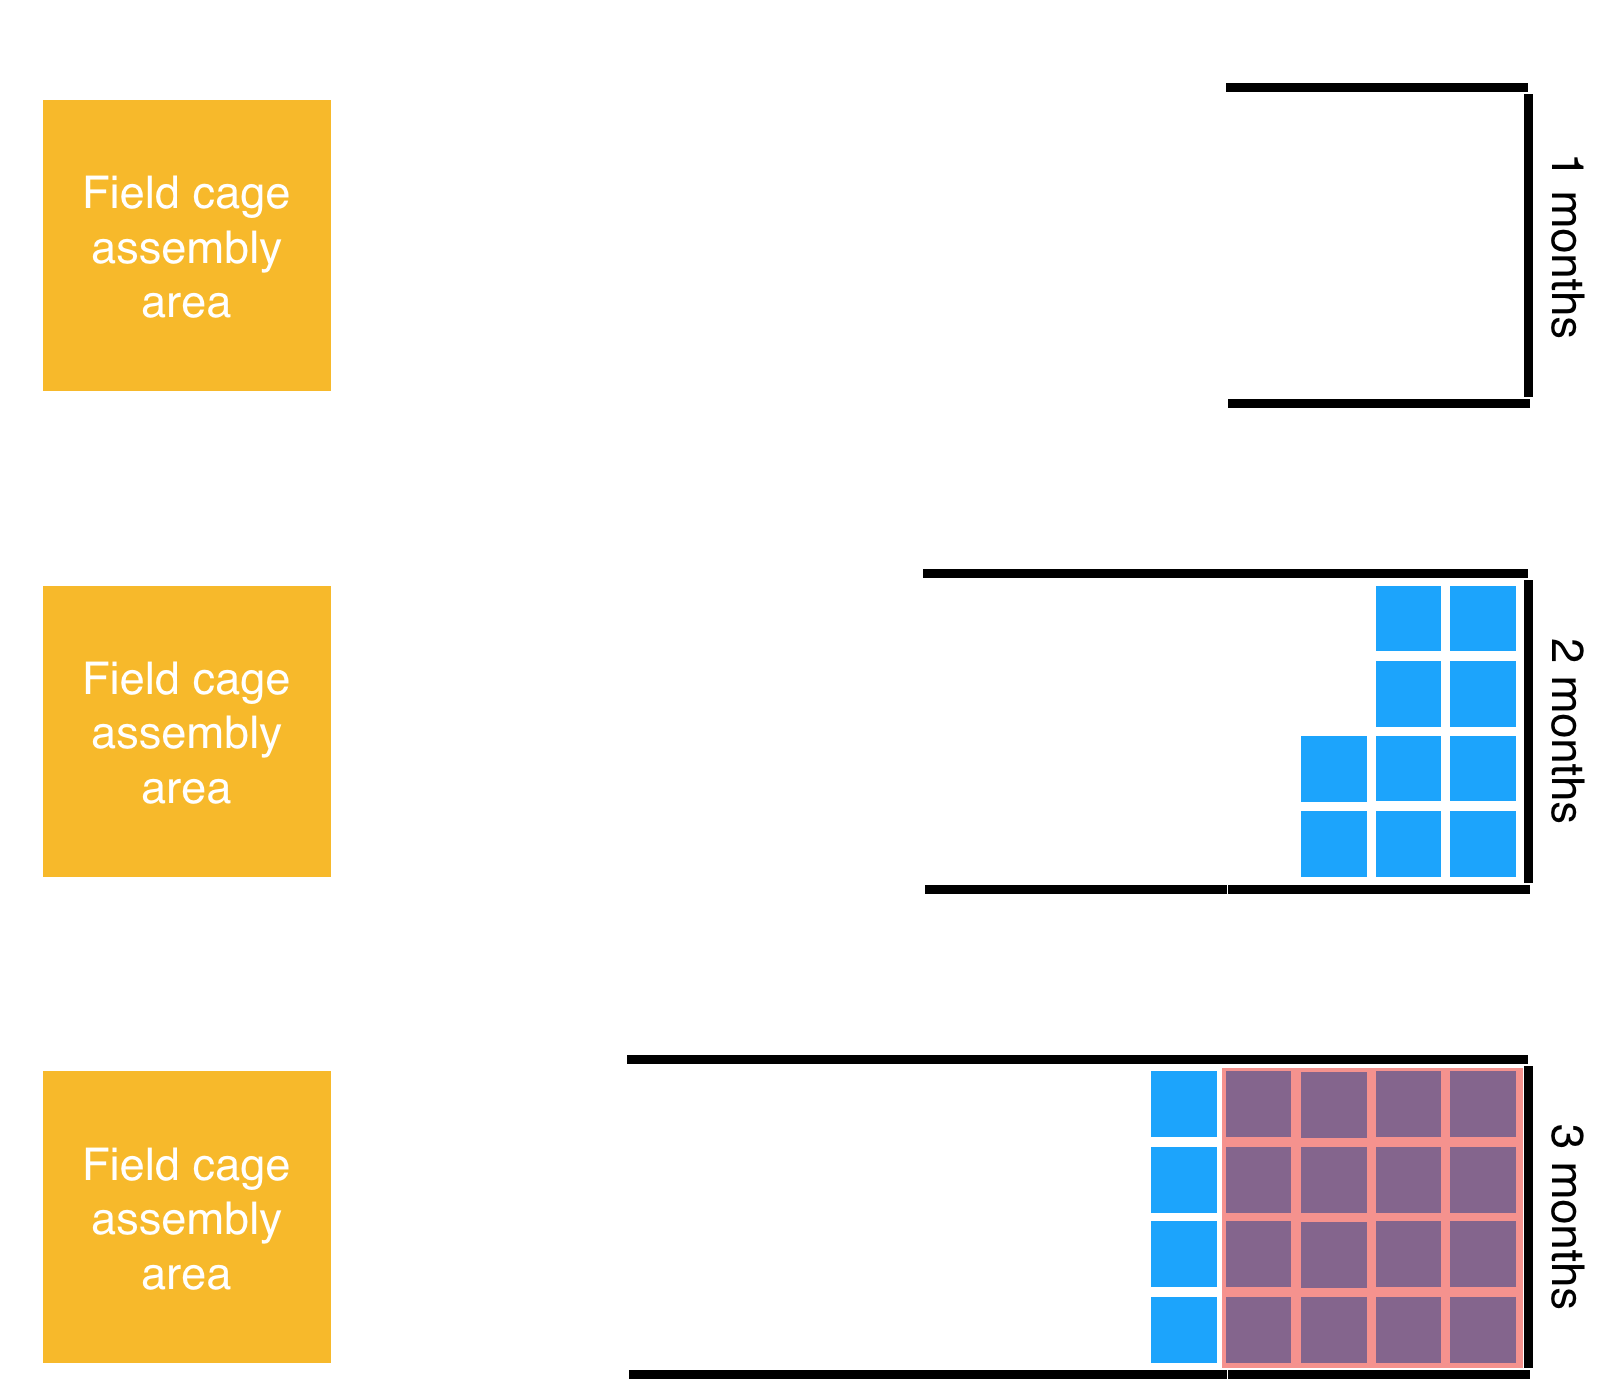
\includegraphics[width=0.5\textwidth]{installationSequence1.png}
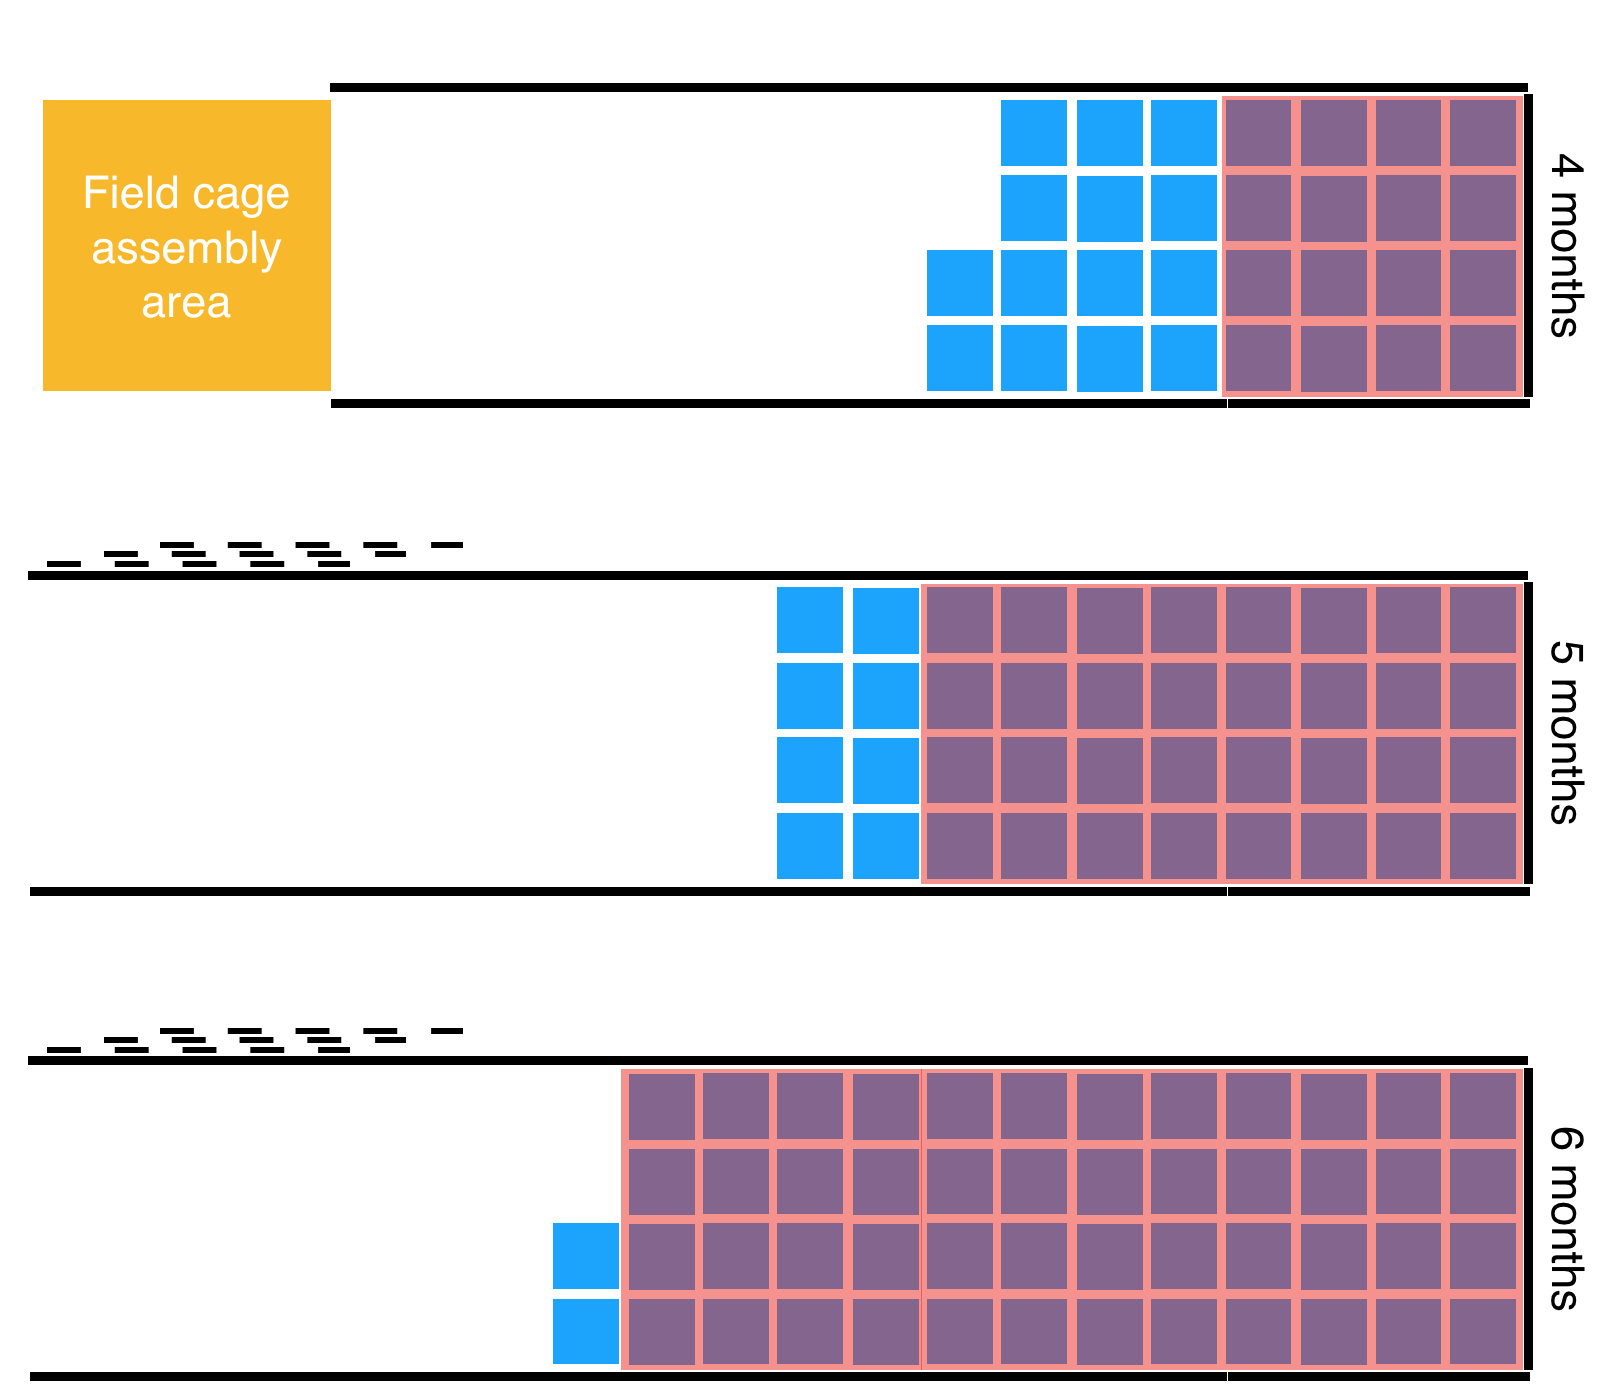
\includegraphics[width=0.5\textwidth]{installationSequence2.png}
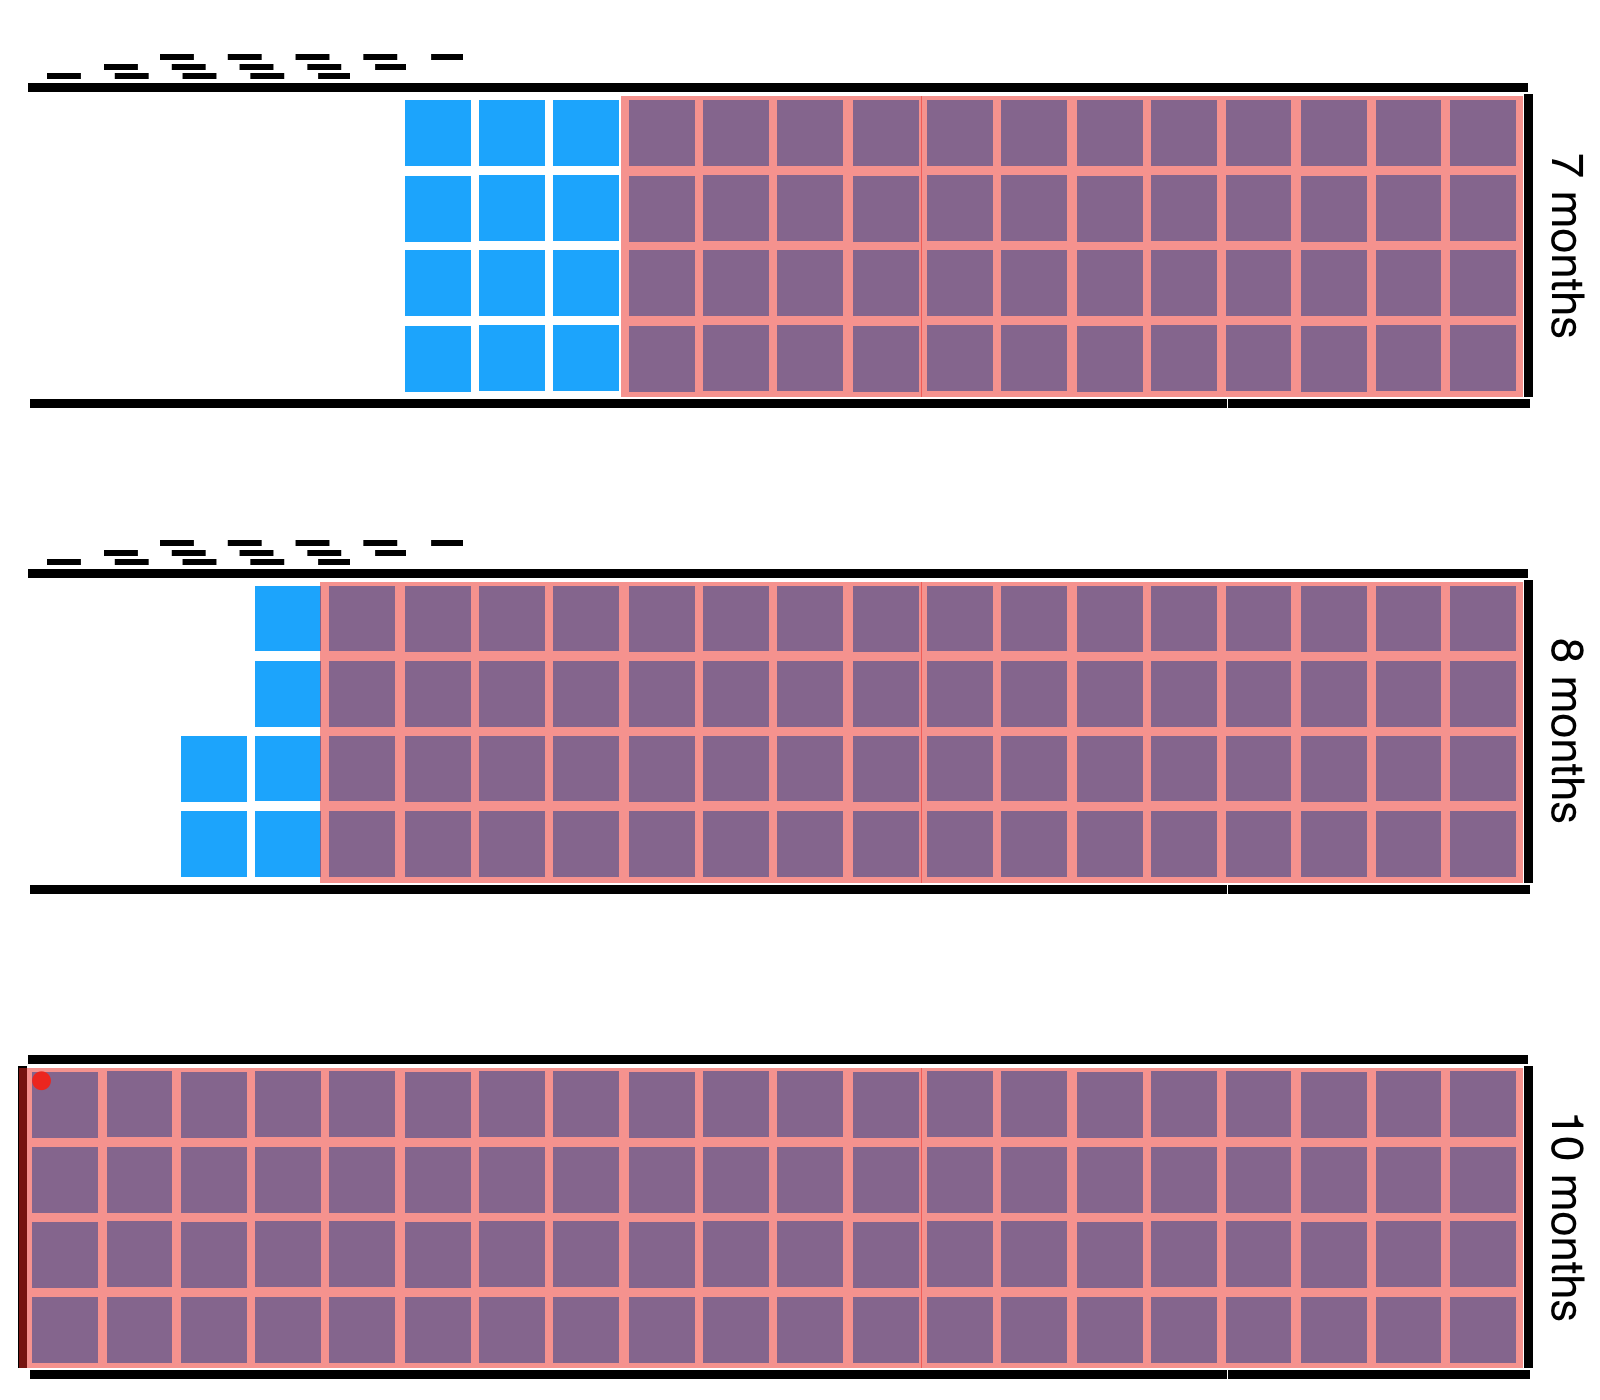
\includegraphics[width=0.5\textwidth]{installationSequence3.png}
\end{dunefigure}

Figure~\ref{fig:globalInstallationSequence} shows the global and overall sequence of installation of the \dword{dp} \dword{tpc}.
The \dword{tco} is on the left side of this sketch.
The orange area is dedicated to the assembly of the \dword{fc}.
This zone is large enough to allow confortably the assembly and the storage of the \dword{hv} system components and the access of material and personnel to the cryostat through the \dword{tco}.
This zone is temporary, and it will be use for the first four months of activities inside the cryostat.
At that time, all the field cage installation will be completed except for the end-wall in front of the \dword{tco}.
The \dword{fc} sub-modules, nonetheless, will be assembled and ready to be installed when needed.
The \dword{fc} installation preceeds always the \dword{crp} installation except for the end-wall on the \dword{tco} side.
The \dwords{crp} are installed at rate of ten \dwords{crp} per month.
The rhythm is dictated more by the  \coldbox tests other than the actual time it takes the to install the \dwords{crp}.
The connection of all the \dword{crp} related cables is the most time consuming and delicate activity.
The finalisation of the \dword{crp} \dword{hv} connection may need extensive work on the cryostat roof, if it is done in the same way as \dword{pddp}.
At roughly the same installation rate, the cathode, the ground grid and the \dwords{pd} are installed.
In this case, the most assembly of the cathode will drive the activities inside the cryostat.
Once the cathode is installed, the ground grids and the \dwords{pmt} installation will flawlessly keep the pace.
The last two busy months of \dword{tpc} installation are dedicated to the completion of the \dword{crp} installation, assembly and installation of the last \dword{fc} end-wall, installation of the cathode, ground grids and \dword{pmt} and the installation of the \dword{hv} extender to connect the \dword{hv} feedthrough to the cathode.


\subsection{Charge readout plane installation}
The \dwords{crp} are transported in a box that make the \dword{crp} assembly a more solid structure, it protects the fragile devices in the \dword{crp}, like the extraction wires, and it keeps it clean.
The size of the transportation boxes is $3.2\times3.5\times0.8$~m$^3$ and it is compatible with the shafts dimensions at \dword{surf}.
The box themselves are protected by a plastic layer that is removed once they arrive in the clean room area underground.
The transportation box is essential for manipulating the \dword{crp} from a vertical orientation (i.e., for storage and for insertion into the temporary construction opening \dword{tco}) to the horizontal orientation, required for the  \coldbox test, lift and final installation.
Once installation is completed, the transportation boxes are wrapped again with a protective layer and shipped back to the production facilities to be re-used.
The \dword{crp} box may need to be modified allowing to stand and mone on wheels when verticall.
This would allow optimisation of the storage on surface and underground.
The \dwords{crp} from the production facilities are shipped to the \dword{sdwf} that act as a buffer zone.
Given the space contraints underground, the \dwords{crp} should be shipped to \dword{surf} when needed.
A buffer of four \dwords{crp} is expected to be always available underground just outside the cean room.
The floor of the cavern in not flat enough to move the \dword{crp} boxes on their wheels.
A dedicated manual or electric transport tool to limit the acceleration and shacking of the \dword{crp} must be used instead.
Once in the clean room, the box can be moved on the wheels.
In order to be efficient in concluding the  \coldbox tests (described later), temporary storage underground for four boxes (vertically) is foreseen.
The boxes are needed to transport the \dwords{crp} from the clod box test into the cryostat.

The sequence of operations inside the cryostat for each \dword{crp} is like the installation sequence followed for the \dword{pddp}:
\begin{enumerate}
\item A \dword{crp} module is brought to the entrance of the cryostat in its transport box.
\item From horizontal position, the box is hung from the side and put it in veryical position to be inserted through the \dword{tco} using the \dword{tco} I-beam.
\item Inside the cryostat, the CRP and its box are laid horizontally and rolled on the false floor to the designated position.
\item The \dword{crp} inside the box is suspended from temporary cables coming down from the chimney.
\item The transport box is dismounted and removed.
\item The \dword{crp} planarity is measured and tuned based on the metrology survey.
Two people for the measurement and two people for tuning are necessary to complete this task in 0.5 shifts.
\item The \dword{crp} is lifted up with the manual or assisted winches. Once in position, the the mechanical stop is assembled. The \dword{crp} is lowered on the mechanical stop.
\item The cabling of the \dword{crp} patch panels to \dword{hv}, signal, and slow control feedthroughs is done.
\item The winch cable is disconnected and the temporary winch removed.
\item The final hanging system is deployed (the bellows is compressed, the cables from the bellows are connected, the compression from the bellows is removed and the bellows attached, the motor is installed on top of the mechanical feedthrough).
\end{enumerate}
Once the installation and the cabling is completed, the lateral and vertical alignment of the \dword{crp} is performed from the cryostat roof with the help of the distance meter measurements and the metrology service.

\begin{dunefigure}[\dshort{pddp} \dshort{crp} installation]{fig:crpInstallation}
{Steps of the installation of the \dwords{crp} in the \dword{pddp}.}
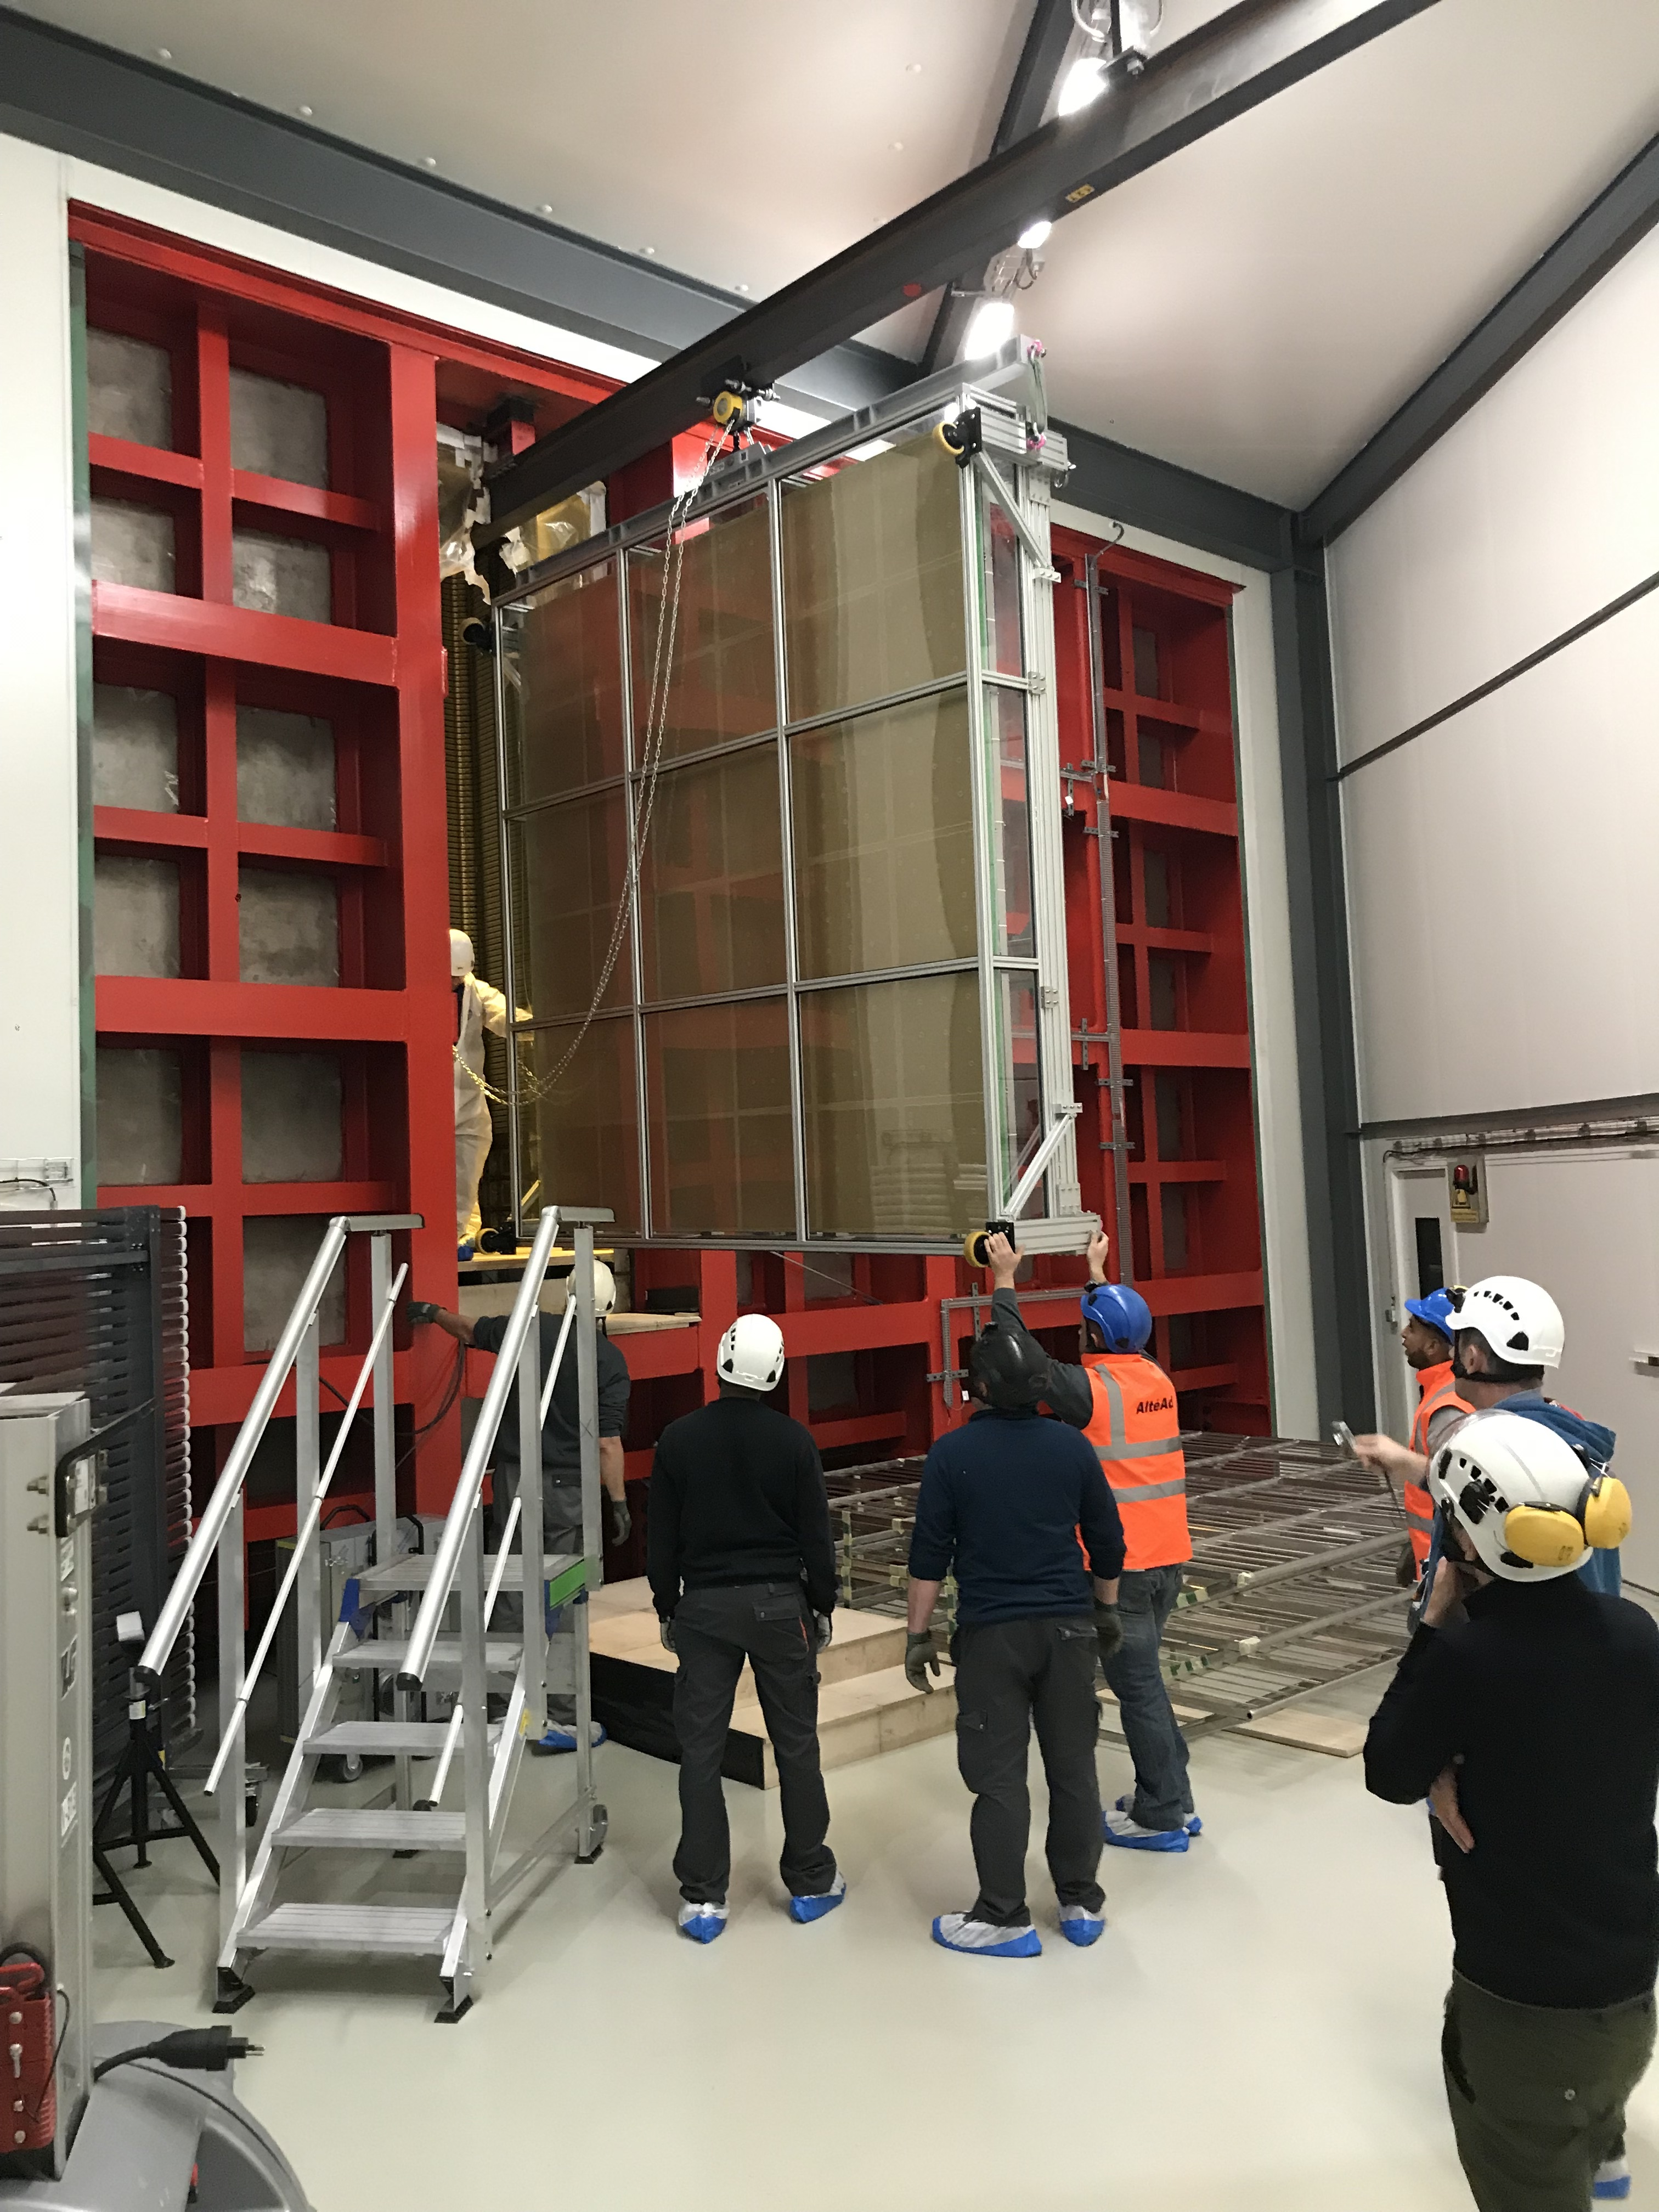
\includegraphics[width=0.45\textwidth]{crpInsertion.jpg}
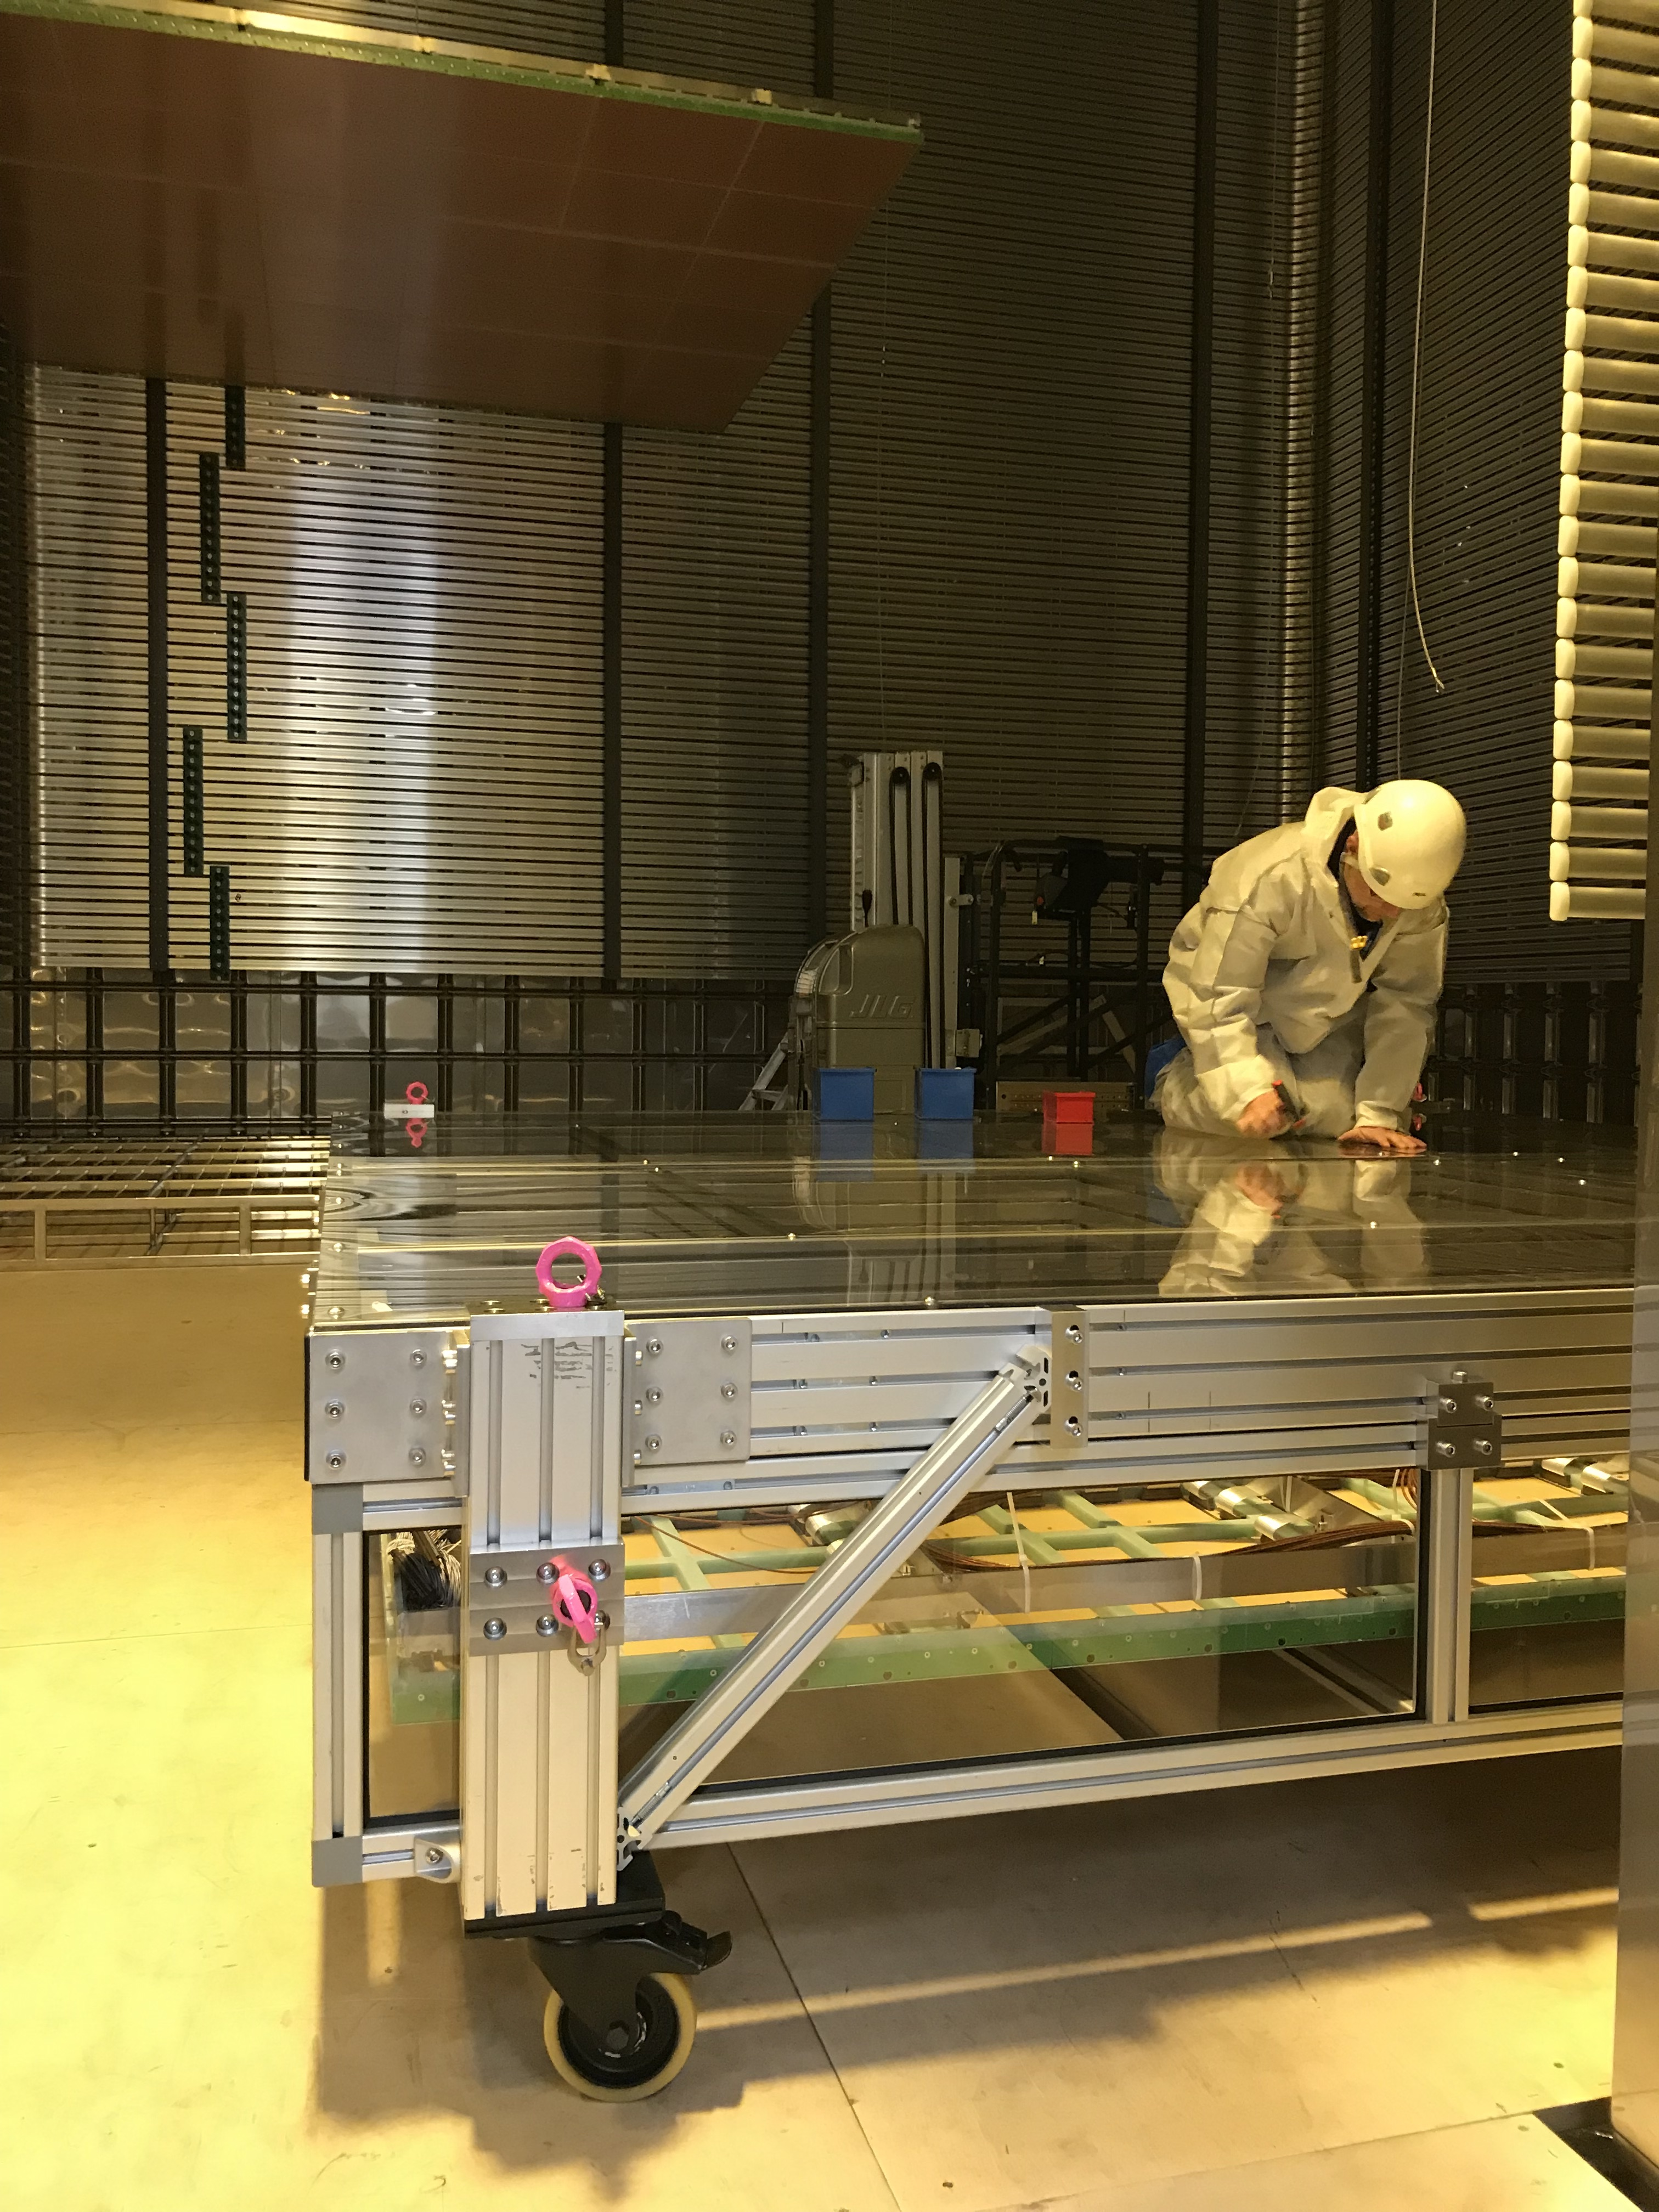
\includegraphics[width=0.45\textwidth]{crpMoving.jpg}
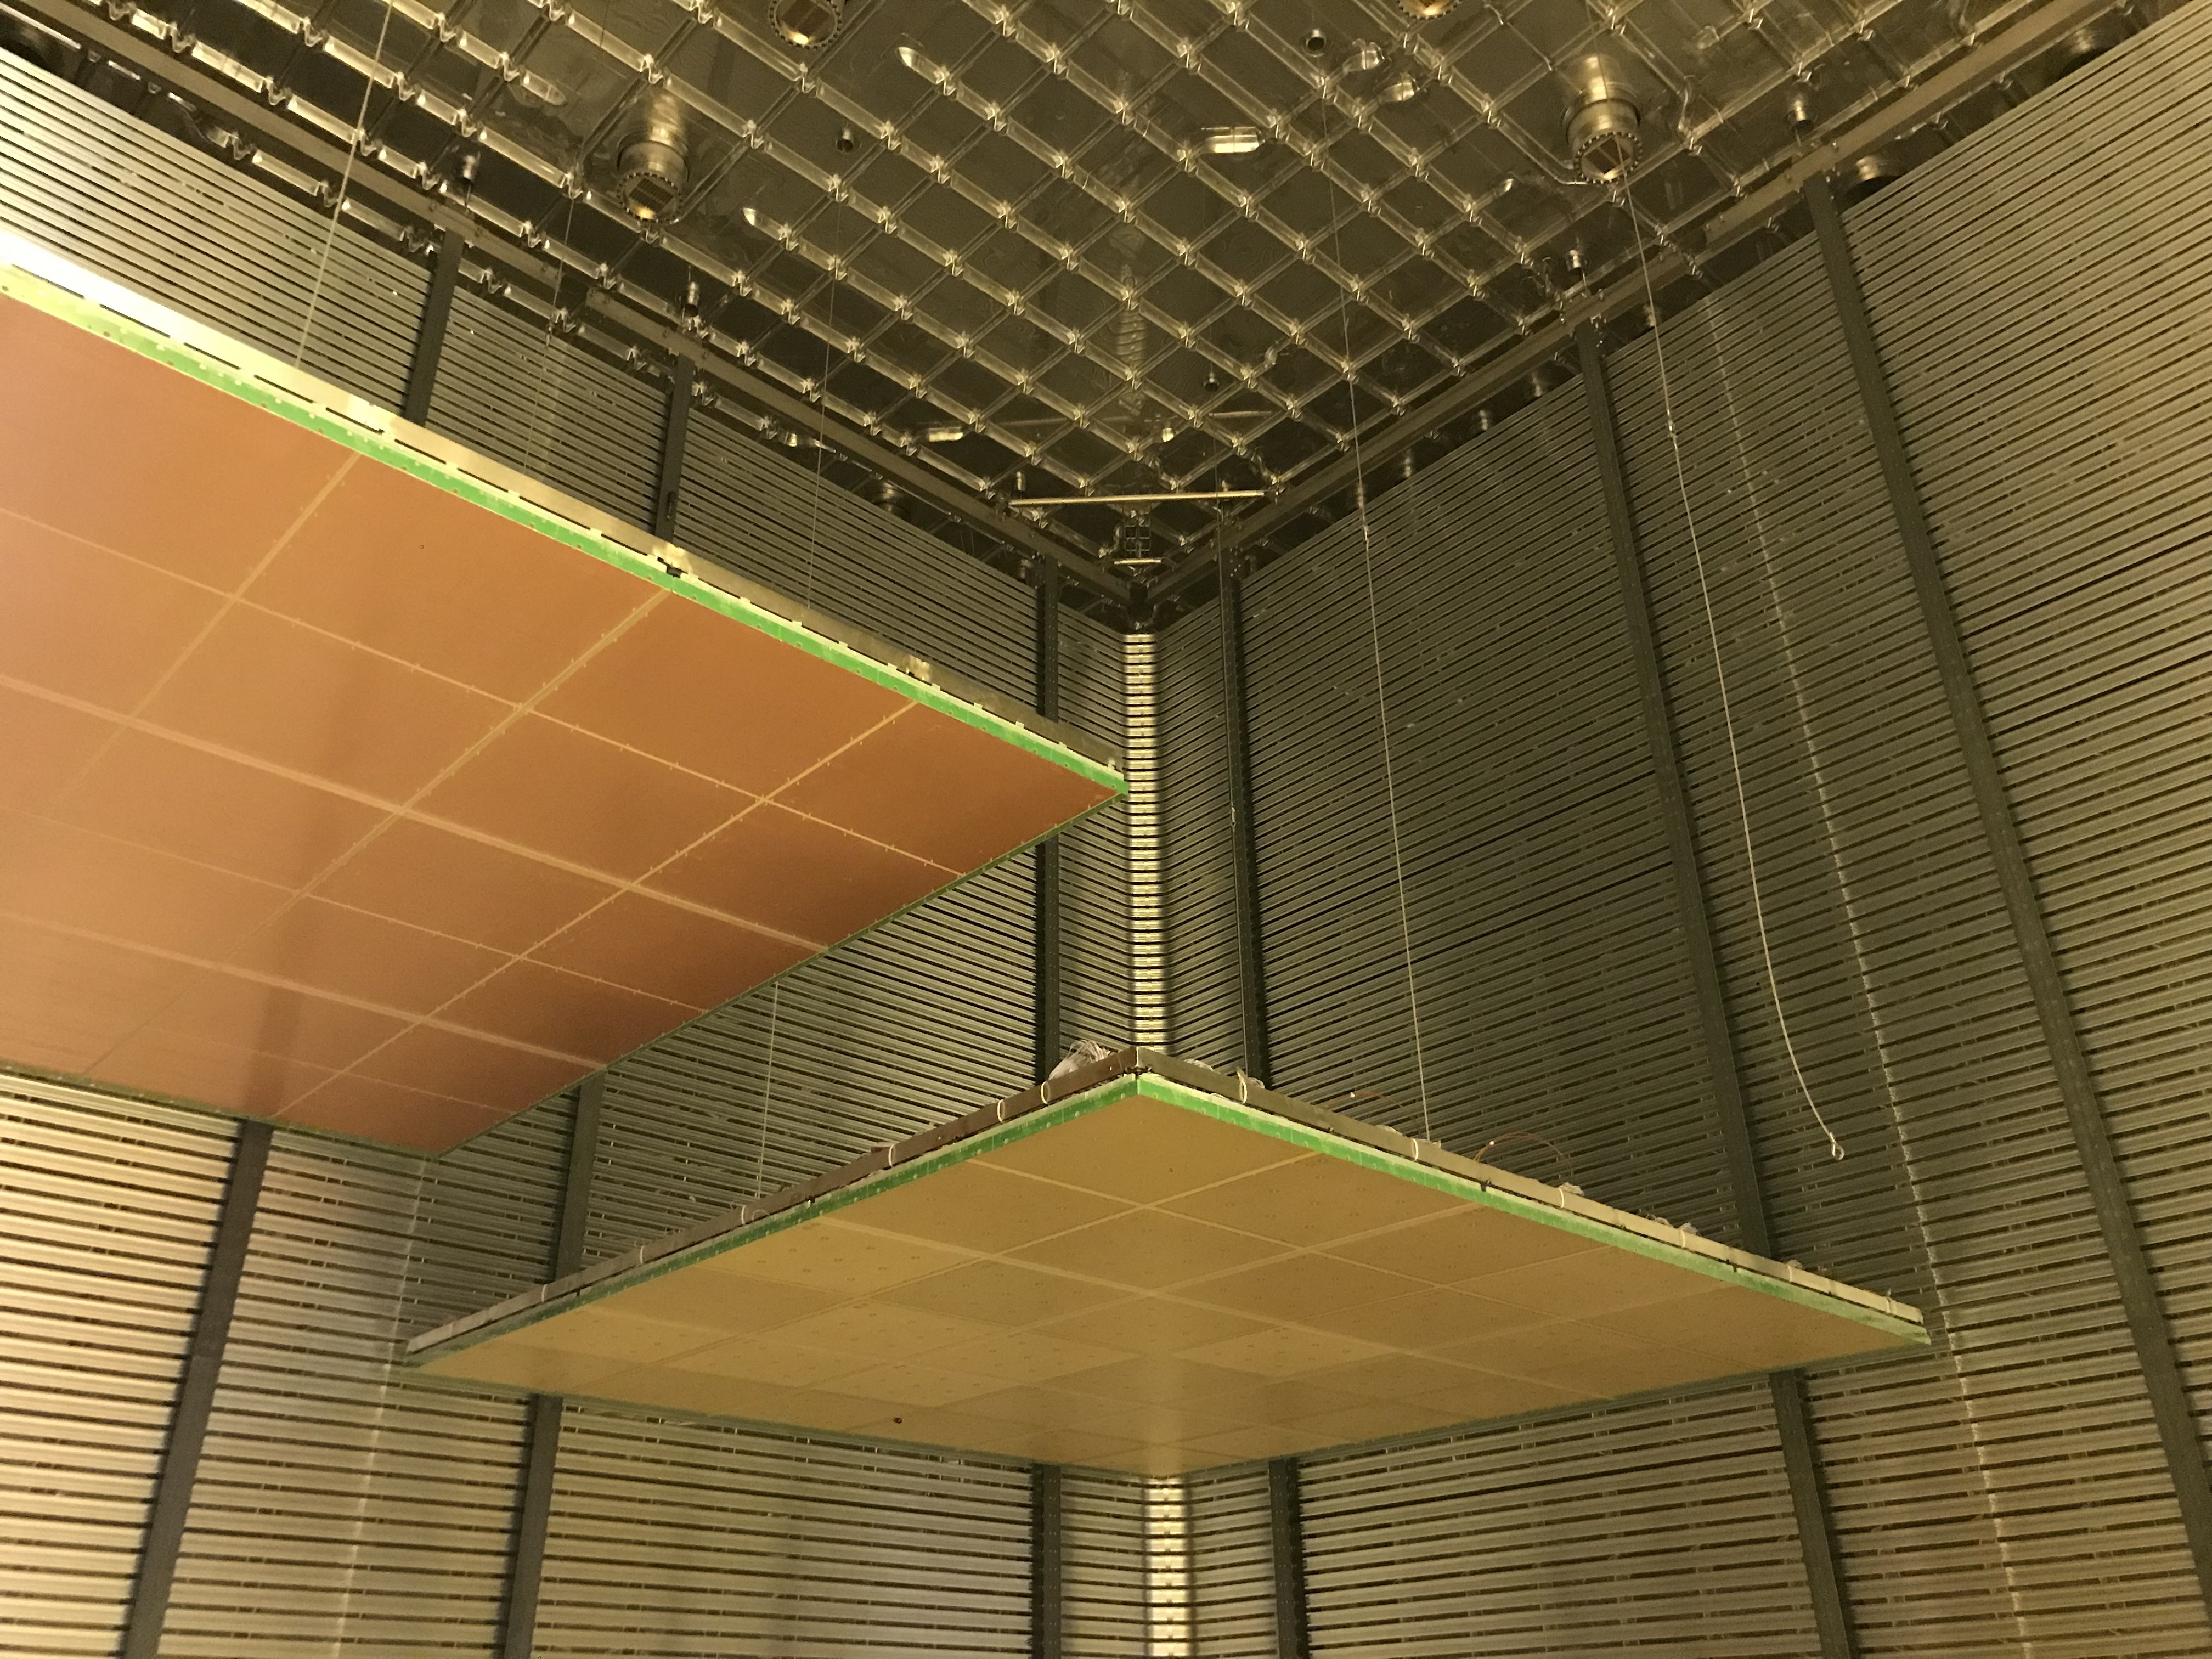
\includegraphics[width=0.9\textwidth]{crpLifting.jpg}
\end{dunefigure}

The installing the 80~\dwords{crp} in the cryostat will take up to ten months.
The signal chimneys underneath the \dword{crp} being installed must be present in order to complete the cabling of the signal cables.
The suspension, instrumentation, and \dword{hv} flanges must also be available.
These components on the roof will be actually installed in parallel with the \dwords{sgft}.
For installation it is foreseen to have enough buffer of \dwords{crp} stored in the vicinity of \dword{surf}.
The installation rate goal is of ten \dwords{crp} installed, cabled, alighted and tested every month.
In order to achieve this goal three teams of two-people in one shift per day are needed.

Provided the means to reach the ceiling for two people, the lifting of one \dwords{crp} in final position is expected to be completed by three people in 0.5 shifts.
The lifting is done from the cryostat roof manually or assisted, depending on the final device available.
The synchronisation of the lifting velocity of the three ropes is fundamental to guarantee the planarity of the \dwords{crp}.
The cabling of the \dwords{crp} is a more complex work.
The position of the \dword{sgft} penetrations and the is \dword{crp} instrumentation penetrations are not always in the optimal position.
The guiding of the cables will be aided by dedicated cable trays and support, but the access, sometimes, will be limited and difficult.
The cabling is done while the \dword{crp} is at the nominal height.
The access between two adjacent CRPs requires staggering the altitude of two neighboring \dwords{crp} for about 20~cm allowing enough space to do the electrical connections.
This procedure was successfully tested and optimized during the installation of the \dword{pddp}.
The cabling must be followed by a scrupulous and prolonged tests of the connections.
This means that even if the final electronics adn power supplies are not finally installed and functional, the \dword{crp} and the cold electronics consortia engages the responsibility of assuring the quality of the connections. 
Optimising the cable bundles one can assume that the cabling of the signal cables for one \dword{crp} is completed by two people in 0.5 shift.
The cabling of the \dword{crp} instrumentation is completed from the inside of the cryostat by two people in 1 shift.
If the \dword{lem} \dword{hv} feedthrough is the same as the one of \dword{pddp}, the finalisation of the connection will take 2 shifts for a person.
The testing of the \dword{lem} \dword{hv} characteristics when installed is a complex issue because the drawn current and the discharge probability depend on the air quality, and above all on the humidity level that at present there is no plan to control.
The \dword{hv} behavior of the installed \dwords{lem} must be followed for a significantly amount of time soon after the installation (days), and repeated regularly.
The first test must be done before the installation of the cathode underneath the \dword{crp} is done: In case of issues the \dword{crp} is reachable without major intervention and disassemble of other detector components.
Therefore, the \dword{hv} tests on the \dwords{lem} are carried on while the \dwords{crp} are still being installed.
A procedure to guarantee the safety of the personnel must still be detailed.
When $4 \times 4$ island of \dwords{crp} are completely installed and before the cathode is in place, a global survey of the 16~\dwords{crp} must be done in order to level them at the nominal position.



Each \dword{crp} will be tested underground in the  \coldbox to characterize its electrical and mechanical behavior in cryogenic conditions.
Figure~\ref{fig:crpTestingSchedule} shows a plausible schedule for tests in the four  \coldbox{}es.
The staggering of the  \coldbox operation is ideal, and very difficult to maintain.
For this reason, the operation of each  \coldbox is meant to be independent.
The time allocated for the opening and the closing procedures is extented by a factor two to compensate possible delays due to activities on two  \coldbox{}es involving the clean room crane at the same time.
In the planing, the installation of the \dword{crp} under the roof of the  \coldbox and the closure of the  \coldbox is allocated in one shift.
Crane drivers (two) will be the main actors in this activity.
From the \dword{pddp} experience, the time it takes to connect the \dword{crp} below the  \coldbox roof, open the transport box, and close the  \coldbox is four hours for two riggers, one \dword{crp} expert, and one technician.
Always based on \dword{pddp} experience, the time allocated for the cool-down and filling of the  \coldbox is two days.
One cryogenic expert is expected to be on shift and supervise the activities for the four  \coldbox{}es (the ability to intervene 24~h/day on cryogenic parameters - most importantly to act on the liquid argon level - is unavoidably).
\dword{crp} and \dword{lem} experts are expected to perform the characterisation in three days.
Two experts per shift will be able to follow the operation of the four  \coldbox{}es.
As in the case of \dword{pddp}  \coldbox tests, during the nights the experts should be able to intervene remotely in case of issues.
The time allocated to empty the  \coldbox and warm it up is two days.
Similarly to the  \coldbox closure, one shift is allocated to open the roof and put the \dword{crp} back in his transport box ready for installation.
One contingency day is considered for each  \coldbox test cycle.
On average 2.5~days will be needed to install and connect the \dwords{crp} inside the cryostat by a group of at least three technicians and one \dword{crp} expert.
An initial period of ramp up, where fewer than four  \coldbox{}es are operational, is expected.
A plausible time line of the number of \dword{crp} tested in each  \coldbox is shown at the bottom of figure~\ref{fig:crpTestingSchedule}.
It is believed that on a schedule of one shift per day seven days per week, the \dwords{crp} will be installed in about 8 months.
The contingency in the test and installation considered in this schedule allow for repairs of minor issues found during the tests.
In the global schedule, the installation of the \dwords{crp} takes 9 months.
This is done to take into account the improbable case where a major issue in up to four \dwords{crp} is found, and these \dwords{crp} must be transported to the surface and shipped back to the factories.
It is also believed that the time needed to test and install the \dwords{crp} will reduced the more \dwords{crp} are tested.

\begin{dunefigure}[Schedule of the \dshort{crp} tests in the \coldbox{}es]{fig:crpTestingSchedule}
{Schedule of the \dword{crp} tests in the four  \coldbox{}es and the number of \dword{crp} tested in each  \coldbox.}
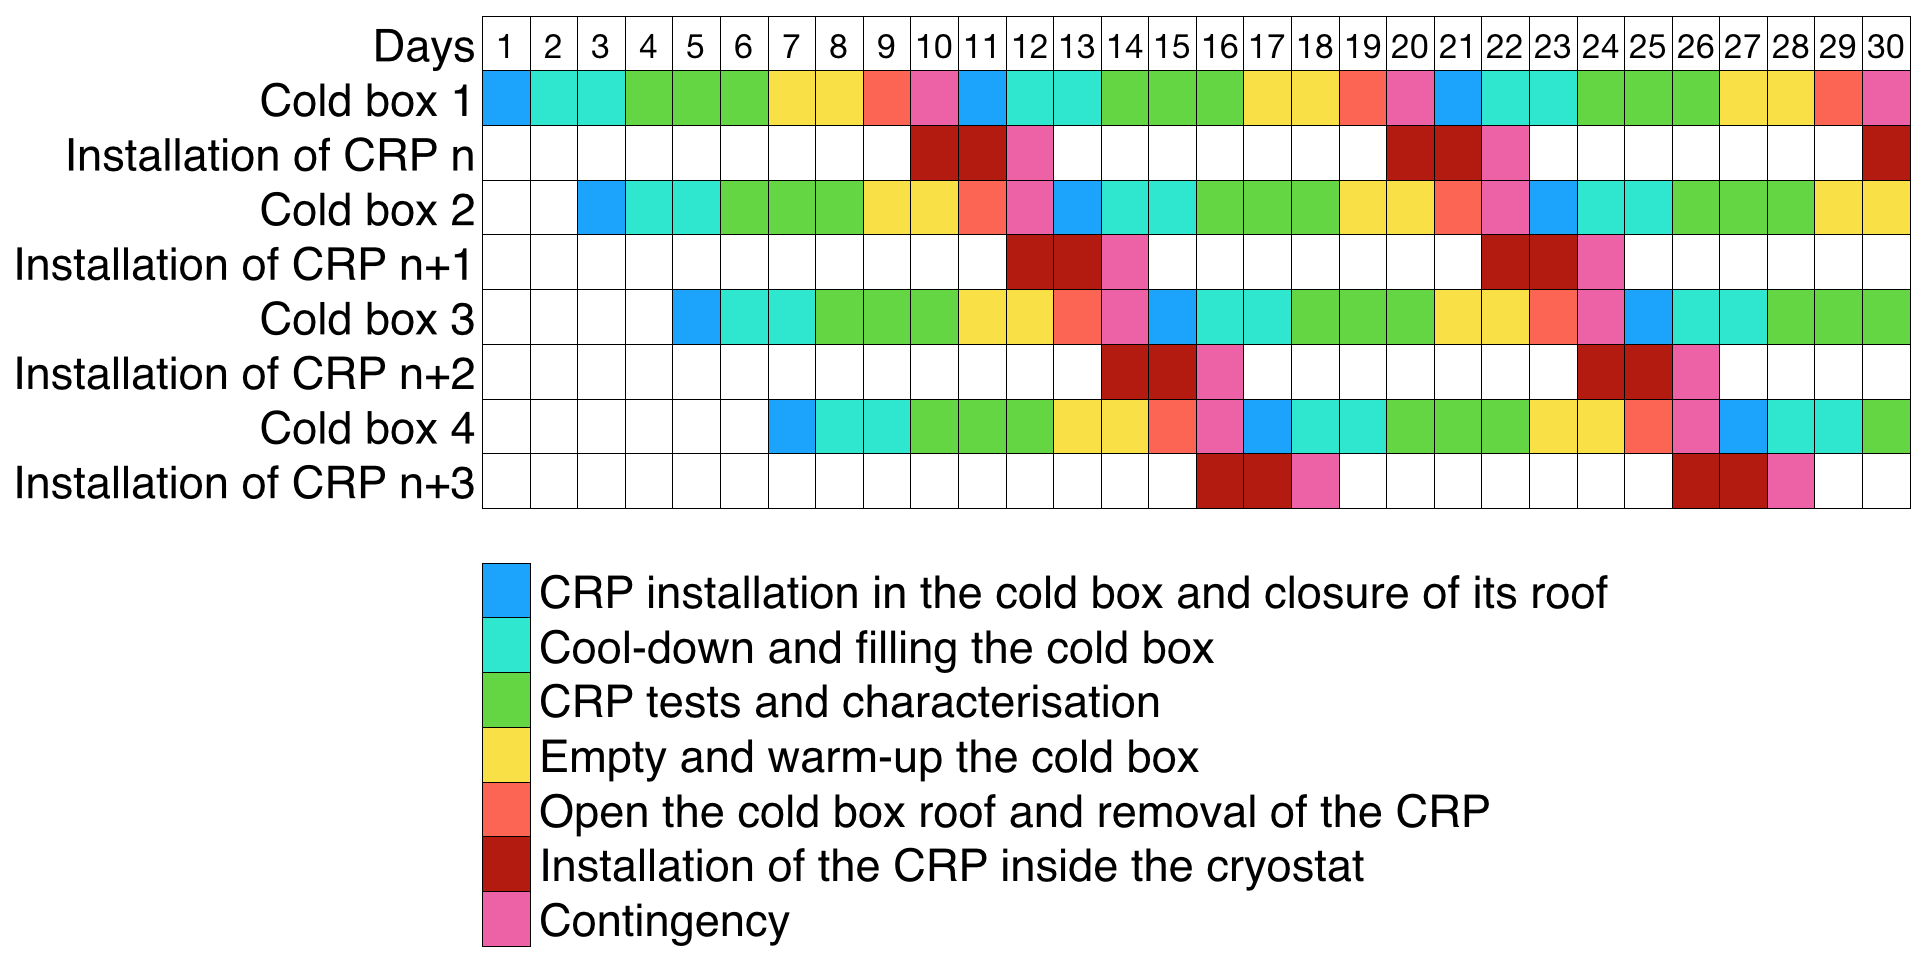
\includegraphics[width=0.8\textwidth]{crpTestingSchedule.png}
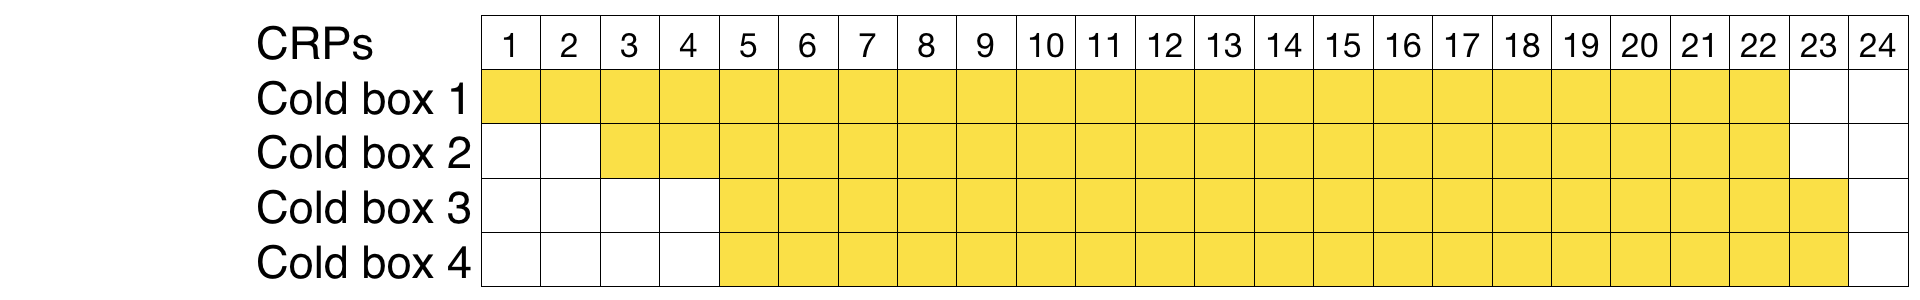
\includegraphics[width=0.8\textwidth]{crpTestDeliveries.png}
\end{dunefigure}


\subsection{High voltage system installation}
Most of the \dword{hv} components installed inside the cryostat will actually be assembled underground.
The reason for this choice is to optimize the transport and storage, considering the fact that the assembly of the \dword{fc} and cathode are not a very resources consuming activities that can be done in parallel with the installation of the \dwords{crp} and \dword{hv} system.

The \dword{fc} \dword{frp} I-beams and the stainless steel cross bars are shipped in standard wooden crates in a very compact fashion.
The components for each \dword{fc} sub-module are packed into one compact flat pack $0.1 \times 0.1 \times 2$~m$^2$ and sealed in several layers of shrink wrap and a thick, soft cushion of plastic layers for edge protection.
Because each sub-module package is so compact, each wooden crate of $1.5 \times 1.3 \times 2.5$~m$^3$ can contain up to 110~sub-module flat packs stacked.
Excluding spares, the total number of sub-module flat packs needed for the entire \dword{fc} is 216, there fore only two crates are needed for a total weight of less than 5~ton, that will be stored underground.

The extruded aluminum profiles for \dword{fc} are shipped separately in standard wooden crates.
In all, 199~4~m-long profiles are needed for each 12~m-long \dword{fc} module, for a total of 7164~profiles to transport underground, excluding spares.
The same number of resistive sheaths are shipped separately.
The 12~m (L) 30~cm (H) 2.5~cm (W) trusses for the cathode modules are shipped to \dword{surf} in transport containers, while the 12~m (L) 2.5~cm (D) resistive rods are shipped in standard wooden boxes.
The installation procedure takes into account the lack of storage space at the 4850~level.
The cathode modules are transported underground in an assigned order, corresponding to their installation sequence starting from the end of the cryostat opposite the \dword{tco}.

The power supply, the \dword{hv} feedthroughs, and \dword{hv} extender are sent to \dword{surf} in standard shipping crates and brought underground when installation requires.

The \dword{fc} is divided in twelve super-module of $12\times12$~m$^2$, five along each long side wall and one along each end-wall.
Each super-module is built out of 18~sub-modules installed in $3 \times 6$ matrix.
The three topmost sub-modules interface with the 12~m-long stainless steel beam from where the entire super-module is hanging.
The three sub-module at the bottom connects with the cathode.

The \dword{fc} sub-modules are assembled inside the \dword{dpmod} cryostat, in a dedicated area of about $5 \times 4$~m$^2$ towards the \dword{tco}.
The completed sub-modules are stored inside the cryostat until they are assembled in the super-module.
The area is large enough for assembly, storage of the sub-modules prior final installation and still allowing comfortably the passage of material and people inside the cryostat.
An assembly table with a precision alignment bar is used for the rapid profile positioning.
The sub-module package is cleaned in the clean room before being brought inside the cryostat by means of the same crane used to insert the \dwords{crp}.
The package is opened on the alignment table and the mechanical frame is assembled from two \dword{frp} I-beams and two stainless steel tubes.
Once the frame is assembled, the aluminum profiles are mounted on the flange of the \dword{frp} I-beams and secured using two slip nuts inserted on either end and are secured with two button-head, hex-drive metal screws, with one side secured tightly and the other loosely, but solidly, in order to avoid stresses due to thermal contraction.
Care must be taken to avoid scratching the profiles during the mounting process.
The resistive sheaths for sub-module interconnections and the square nuts to hold \dword{hvdb} are pre-inserted to each profile at the assembly stage.
All the screws are tightened with the right and reproducible torque using a power screwdriver with a preset torque.
A base with wheels constructed out of unistrut bars is mounted to the bottom of the sub-module, to allow easy handle and transport inside the cryostat to the designated installation section.

When three top sub-modules, three bottom sub-modules, and twelve middle sub-modules are assembled, they will be installed as a super-module starting at the far end of the cryostat.
The installation sequence is thought to avoid the need of working an height higher than 3~m.
The installation for a super-module follow the following steps:
\begin{enumerate}
\item Hang the 12~m-long stainless steel I-beam from two stainless steel cables through the feedthroughs and lift it to approximately 2.5~m above the temporary floor and secure it at this position.
The lift is done from the roof of the cryostat with manual winches in a similar way as done for the \dwords{crp}.
The team inside the cryostat will guide the lifting operation of the team on the roof.
Effective communication between the inside and outside of the cryostat is crucial for this operation.
Walkie-talkies were effectively used for this purpose during \dword{pddp} installation.
Before the stainless steel I-beam is transported inside the cryostat they are cleaned in the clean room.
The time spent inside the clean room is less than 0.5 shift.
The ongoing activities in the celan room should therefore not be perturbated by the cleaning and insertion of the I-beam inside the cryostat, provided that this operation should not be done when the  \coldbox{}es are opened or closed.
The stainless steel I-beam is transported inside the cryostat as for all the other items, and it is transported in the installation point by means of carts rolling on the false floor.
\item Place three top sub-modules under the stainless steel I-beam and connect each to the I-beam using two sets of stainless steel L-brackets, stainless steel inserts, stainless steel screws, stainless steel lock washers, and stainless steel nuts.
\item Slide the two resistive sheaths (pre-inserted into the middle sub-module) over and tighten them onto the two neighboring profiles to make the resistive connections between profiles in the same row.
\item Mount \dword{hvdb} to the center sub-module in the row, using aluminum button-head screws and a square nut pre-inserted in the profile reinforcement rail.
This operation completes one row of the sub-modules for a super-module.
\item Mount the reflector/\dword{wls} panels for the photon detection system to cover completely the first row of sub-modules towards the active volume.
\item lift the completed top row by approximately additional 2.5~m and secure the super-module in this position.
Place three middle sub-modules under the top row, and connect each to the corresponding top sub-module above using 1~cm thick connection plates and stainless steel screws and nuts.
Repeat the relevant steps described above to install all the six raws of sub-modules.
The first three are equipped with the reflectors.
\end{enumerate}

Work at the level of the cryostat ceiling is required in order to connect the super-module to the final anchoring system and release the temporary lifting ropes.
This operation can be done from the inside of the active volume using the man lift as long as the \dwords{crp} in that region are not installed.
Additional work at height is needed to connect the safety ground connection of the topmost field shaping ring with the cryostat wall/ceiling and to connect the topmost field shaping ring power to the dedicated feedthrough port.
Again this activity should be done as last steps of the installation of the super-module with a man lift.

Figure~\ref{fig:fieldCageInstallation} shows a moment in the installation of the \dword{fc} in the \dword{pddp}.
For what concerns the installation sequence, the most relevant difference between the \dword{pddp} (other than the total height of the modules) is the fact that the super-module consisted of one single raw of sub-modules.
In figure~\ref{fig:fieldCageInstallation} the super-modules are still hanging from the temporary lifting stainless steel ropes.
The wheel base carts below the sub-modules are visible.
\begin{dunefigure}[\dshort{pddp} field cage installation]{fig:fieldCageInstallation}
{Installation of the \dword{pddp} field cage.}
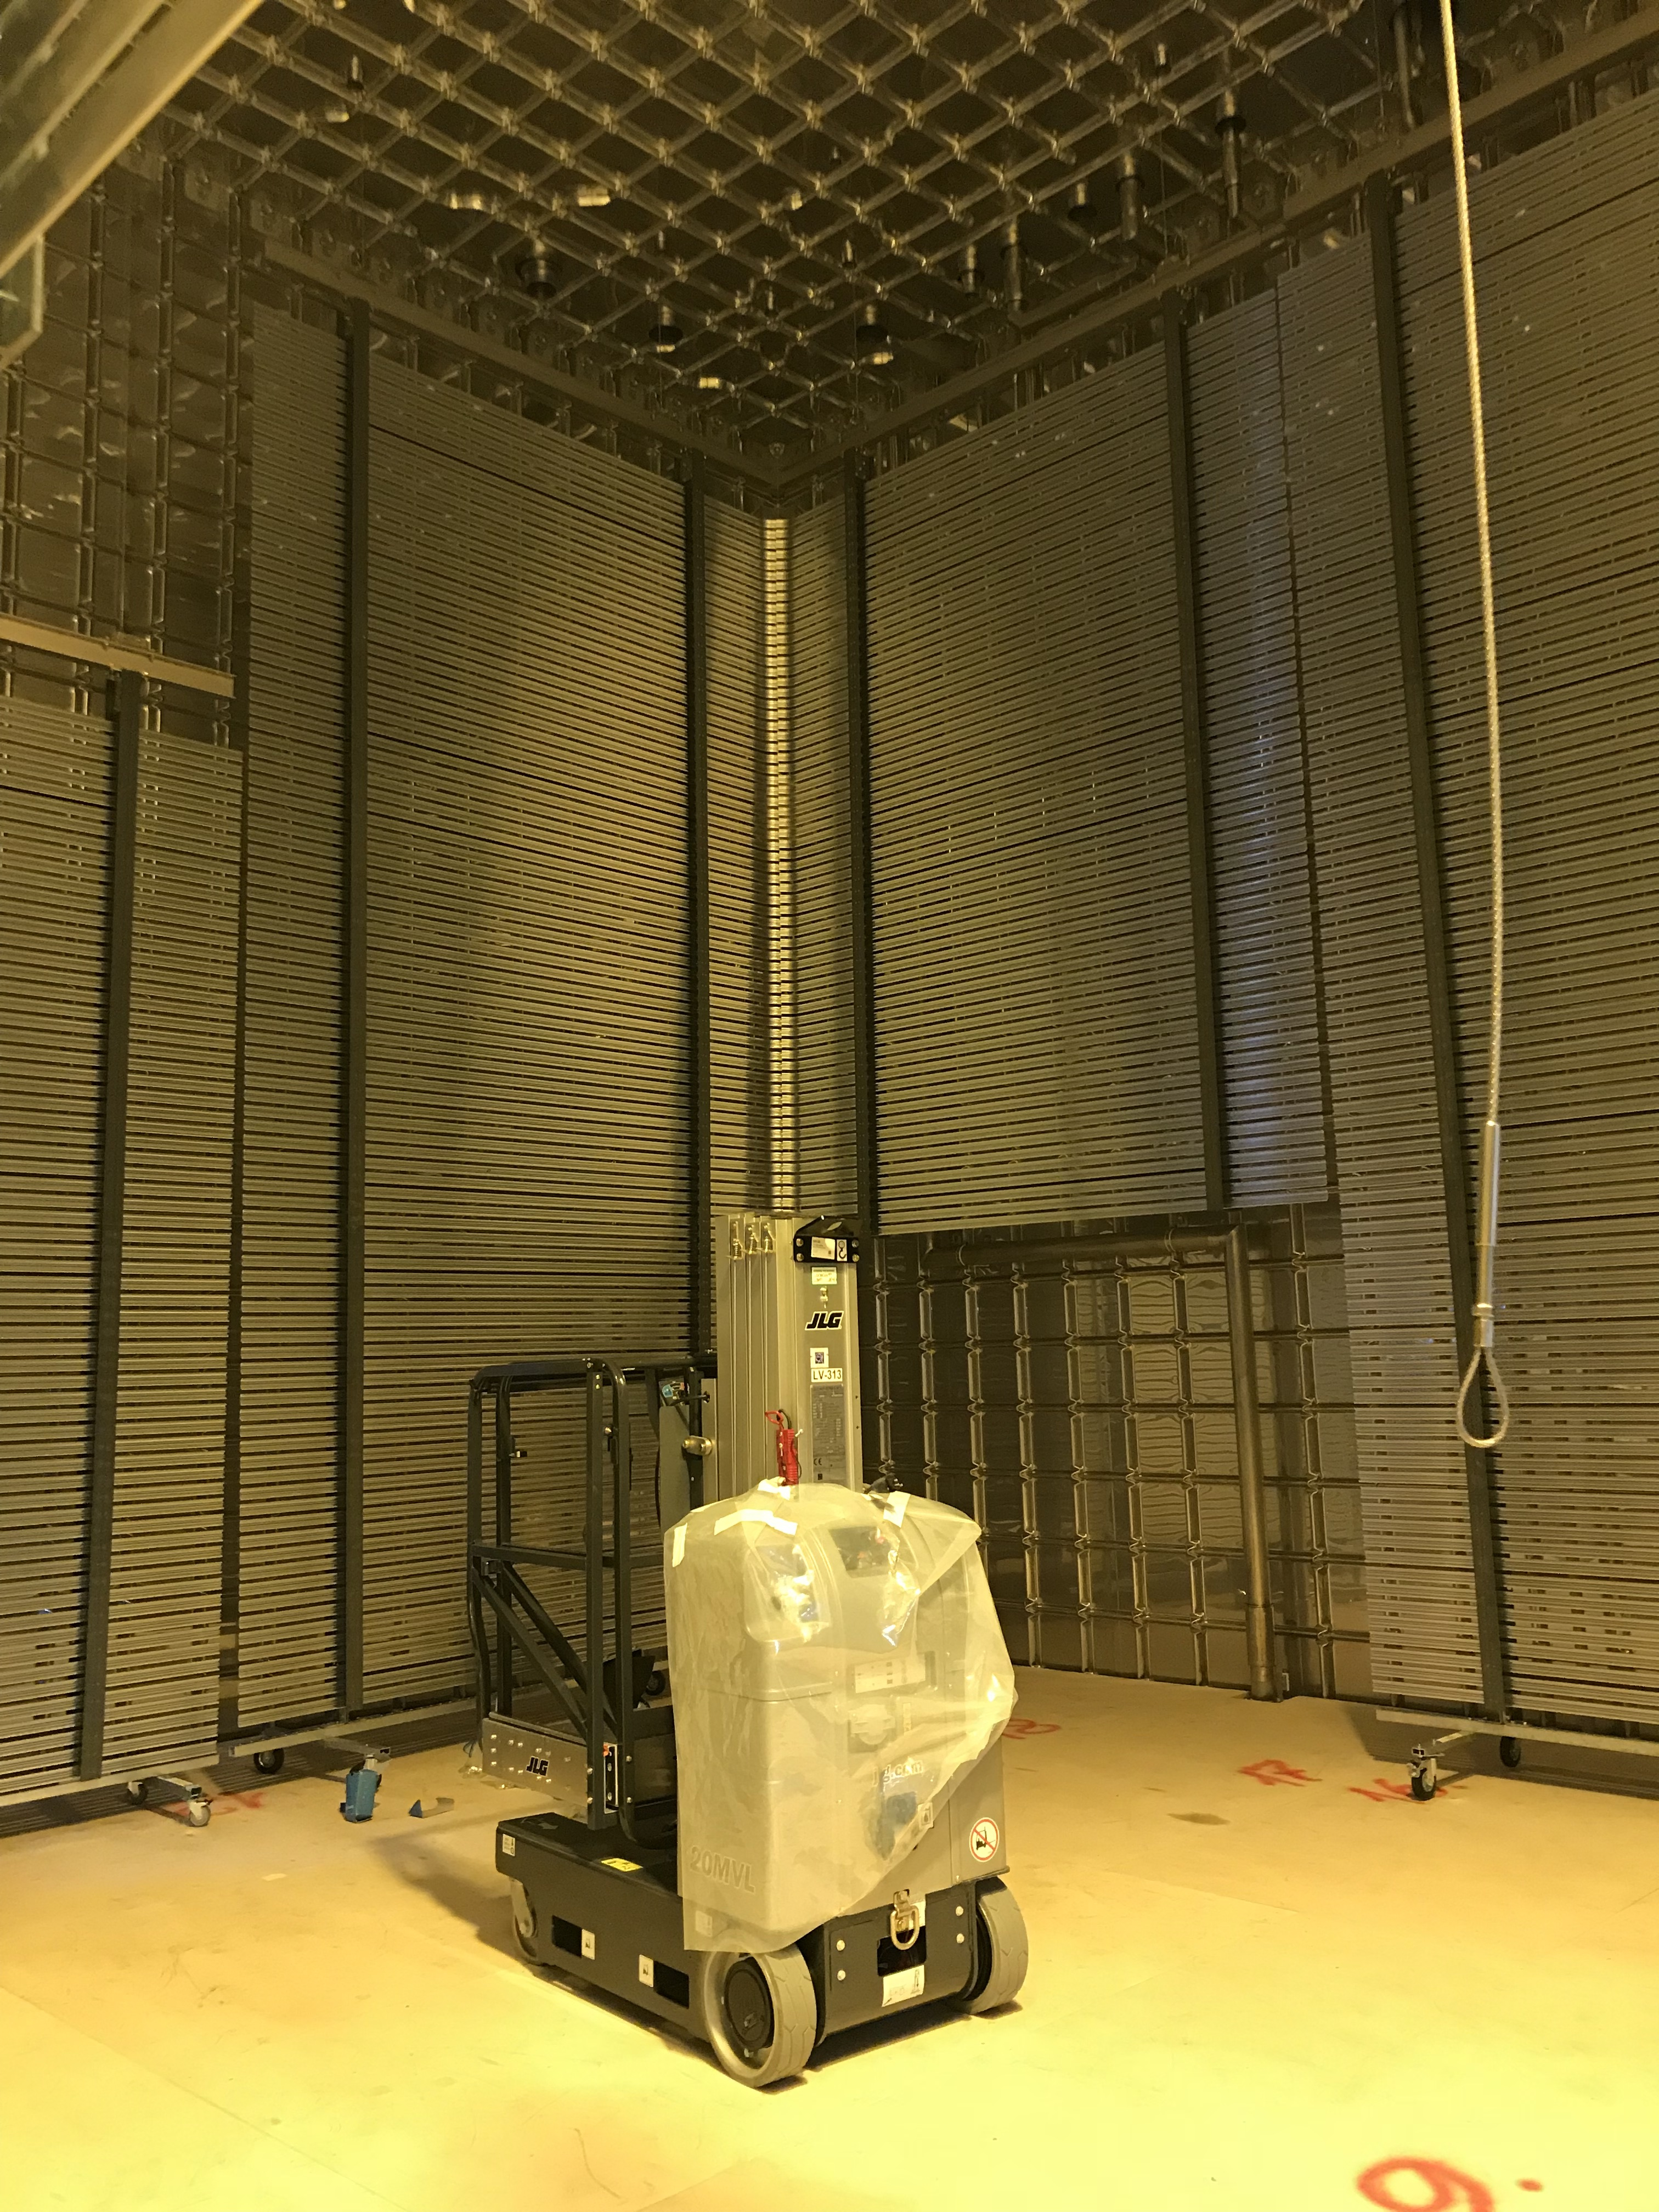
\includegraphics[width=0.9\textwidth]{fieldCageInstallation.jpg}
\end{dunefigure}

The cathode consists of 15~sections of $4 \times 12$~m$^2$ to cover the length of 60~m of the \dword{dpmod} \dword{tpc}.
They are installed hanging from the bottom of the \dword{fc} connecting the two long walls.
Each section consists of two 12~m-long trusses made from thin-walled stainless steel tubes with approximately 50~mm outer diameters.
They can either be prefabricated and transported underground like the large cryostat I-beams or assembled in the underground area from sectional parts.
They must be un-boxed and cleand inside the clean room before entering into the cryostat.
The trusses are 2~m apart and are connected at both ends to stainless steel tubes that run under the \dword{fc} and form the outer tube ring of 144~m surrounding the cathode plane.
The actual cathode plane consists of 10~mm diameter resistive rods installed at a pitch of 10~cm through holes in the straight upper tubes of the trusses.
The \dword{fc} end-wall must be pushed about 50~cm towards the inside of the active volume to meet the \dword{fc} side walls and cathode to form a trapezoidal section of the active volume.
This is required to move away the cathode from the cryostat walls and meet the maximum field specification inside the liquid argon.

The ground grid that protect \dwords{pd} from the high electric field consists of 80~self sustained modules made out of stainless steel.
They are installed with four legs directly on the corrugated floor with teflon sheets to protect it from scratces.
The legs can be extended to allow confortably the installation of the \dwords{pd}.
The position of the legs matches the flat part of the corrugation adn avoid the \dwords{pd} and the internal cryogenic lines.
The ground grids are light enough that can be transported and handled manually by two people and installed by four people.
For more details see the \dword{hv} chapter of this \dword{tdr}.

The entire \dword{hv} system, including \dword{fc}, cathode, ground grid, and the reflector/\dword{wls} panels are installed in the following sequence:
\begin{enumerate}
\item Construct the end-wall super-module (equipped with the 90~degree bent corner profiles) at the end of the cryostat opposite to the TCO.
\item Mount the U-shaped stainless steel cathode end-wall perimeter tube to the bottom of the end-wall super-module.
\item Install the two super-modules along the side wall immediately next to the end-wall module.
\item Make the electrical connections to the end-wall super-module.
\item Pull in the bottom of the end-wall super-module about 50~cm from its free hanging position in order to align its profiles to the ones of the wall \dword{fc} super-modules. Secure the end-wall super-module to the temporary false floor.
\item Electrically connect the end-wall super-module and side wall super-modules using the pre-inserted resistive sheath.
\item Assemble the cathode module in place at the bottom of the two side \dword{fc} modules immediately next to the end-wall super-module.
Special lifting equipment is foreseen to manipulate the cathode and lift it in position to allow simple connection to the~\dword{fc}.
\item Connect the stainless steel perimeter cathode tube already mounted on the end-wall super-module to the corresponding cathode tubes on the side wall super-modules, and anchor it to the false floor to ensure the mechanical stability of the end-wall super-module until the entire \dword{fc} is constructed.
\item Once the cathode section is securely hanging from the \dword{fc}, remove the temporary floor under the cathode, and clean the membrane floor.
\item Place the ground grids under the cathode plane with their legs extended and start the installation of the \dwords{pmt}.
\item Once the \dwords{pd} installation is completed and cabling is complete below one ground grid, remove the leg extensions of the ground grid and lower it to the nominal height.
\end{enumerate}
Figure~\ref{fig:groundGridInstallation} shows the installation in \dword{pddp} of the ground grid above the \dwords{pmt} already in final position.
In this case, four $3 \times 3$~m$^2$ sections of the ground grid where installed.
The sections had to be connected to each other, they where not independent.
From the installation point of view ground grid in the \dword{dpmod} will be simpler to install compared to the \dword{pddp} also because the ground grid frame between the cryostat walls and the main ground grid, present in \dword{pddp}, will not be installed in \dword{dpmod}.

\begin{dunefigure}[Installation of the ground grid above the \dshorts{pmt} in the \dshort{pddp}]{fig:groundGridInstallation}
{Installation of the ground grid above the \dwords{pmt} in the \dword{pddp}.}
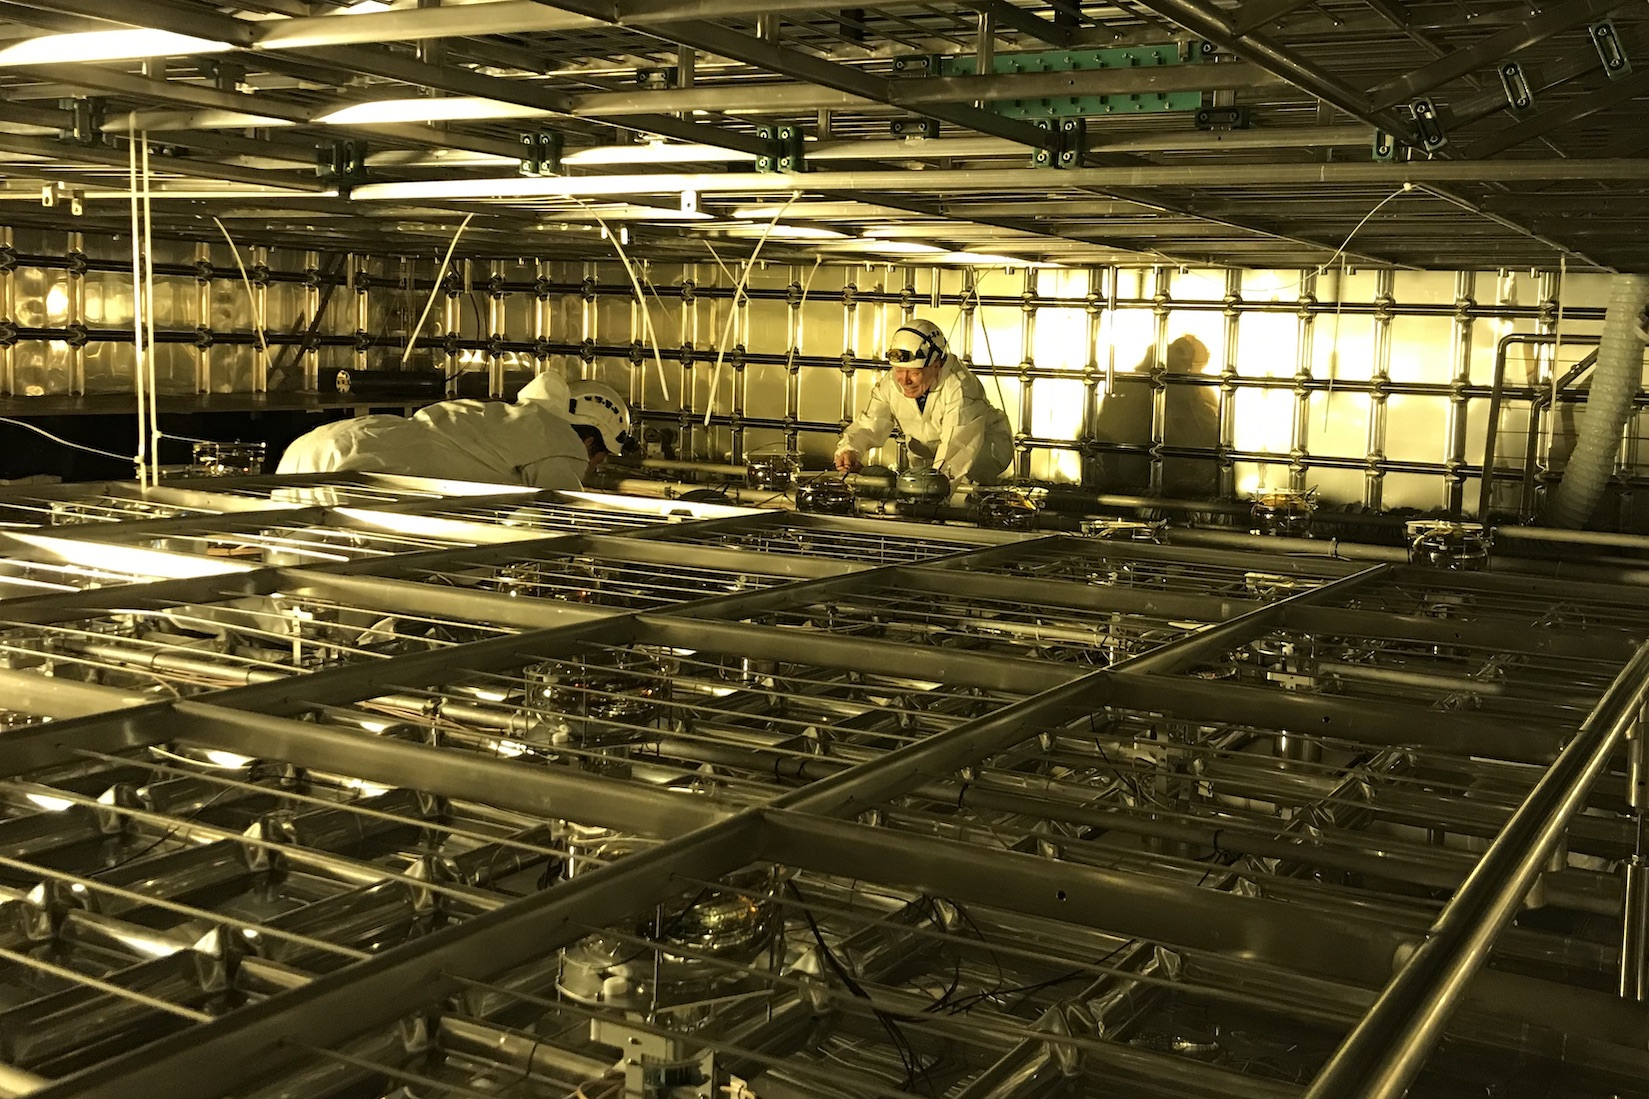
\includegraphics[width=0.9\textwidth]{groundGridInstallation.jpg}
\end{dunefigure}

What was described above is the procedure that is valid until the installation of the \dword{tco} end-wall.
To assemble the end-wall super-module as the others, all the \dwords{crp} must be installed first and all the sub-modules for the last super-module must be available inside the cryostat stored on the false floor around the active volume.
The man lifts needed for the installation of the \dwords{crp} are too tall to pass below a fully installed end-wall to being finally extracted from the cryostat.
In \dword{pddp} the bottom-most sub-module of the super-module in front of the \dword{tco} was not installed.
This was possible because the super-module consisted of a single raw of sub-modules.
The activities at the ceiling level for what concerns the last end-wall will be carried out using a scaffold.
Once the end-wall is in place, the \dword{hv} extender that that was inserted into the cryostat prior the installation of the end-wall,
is installed.
As per the actual design, the extender is a 12~m-long rigid cylinder with an inner conductor and outer field shaping rings.
Its role is to create an electrical connection between the tip of the feedthrough, that is installed as last thing, and the cathode without too much distorting the drift field in its vicinity and guaranteeing a maximum electric field inside the liquid argon below 30~kV/cm.
For the installation, the extender (unpackedn and cleaned) is laid horizontally on a portion of false floor left free of the scaffold.
It is lifted vertically with a pulley and a rope passing through the \dword{hv} feedthrough.
It is finally secured to the anchoring mechanism welded on the penetration pipe.
The extender pass through a special \dword{crp} that leaves a corner without anode, \dwords{lem}, grid or any other mechanical obstacles.
Figure~\ref{fig:extenderInstallation} shows this operation done in the \dword{pddp} with the 6~m-long extender, which in that case was installed outside the active volume (no special \dword{crp} was needed).
Once all the electrical connections of the \dword{hv} system are established, a global continuity test will be conducted applying voltage at the cathode through the \dword{hv} feedthrough and measuring the current drawn.
Monitor the voltage and current will be an exercise repeated regularly before the beginning of the gas argon purge, and it will constantly done during purge, cool-down and filling. 
\begin{dunefigure}[Installation of the \dshort{hv} extender in the \dshort{pddp}]{fig:extenderInstallation}
{Lifting of the \dword{hv} extender from horizontal to vertical position in the \dword{pddp}.}
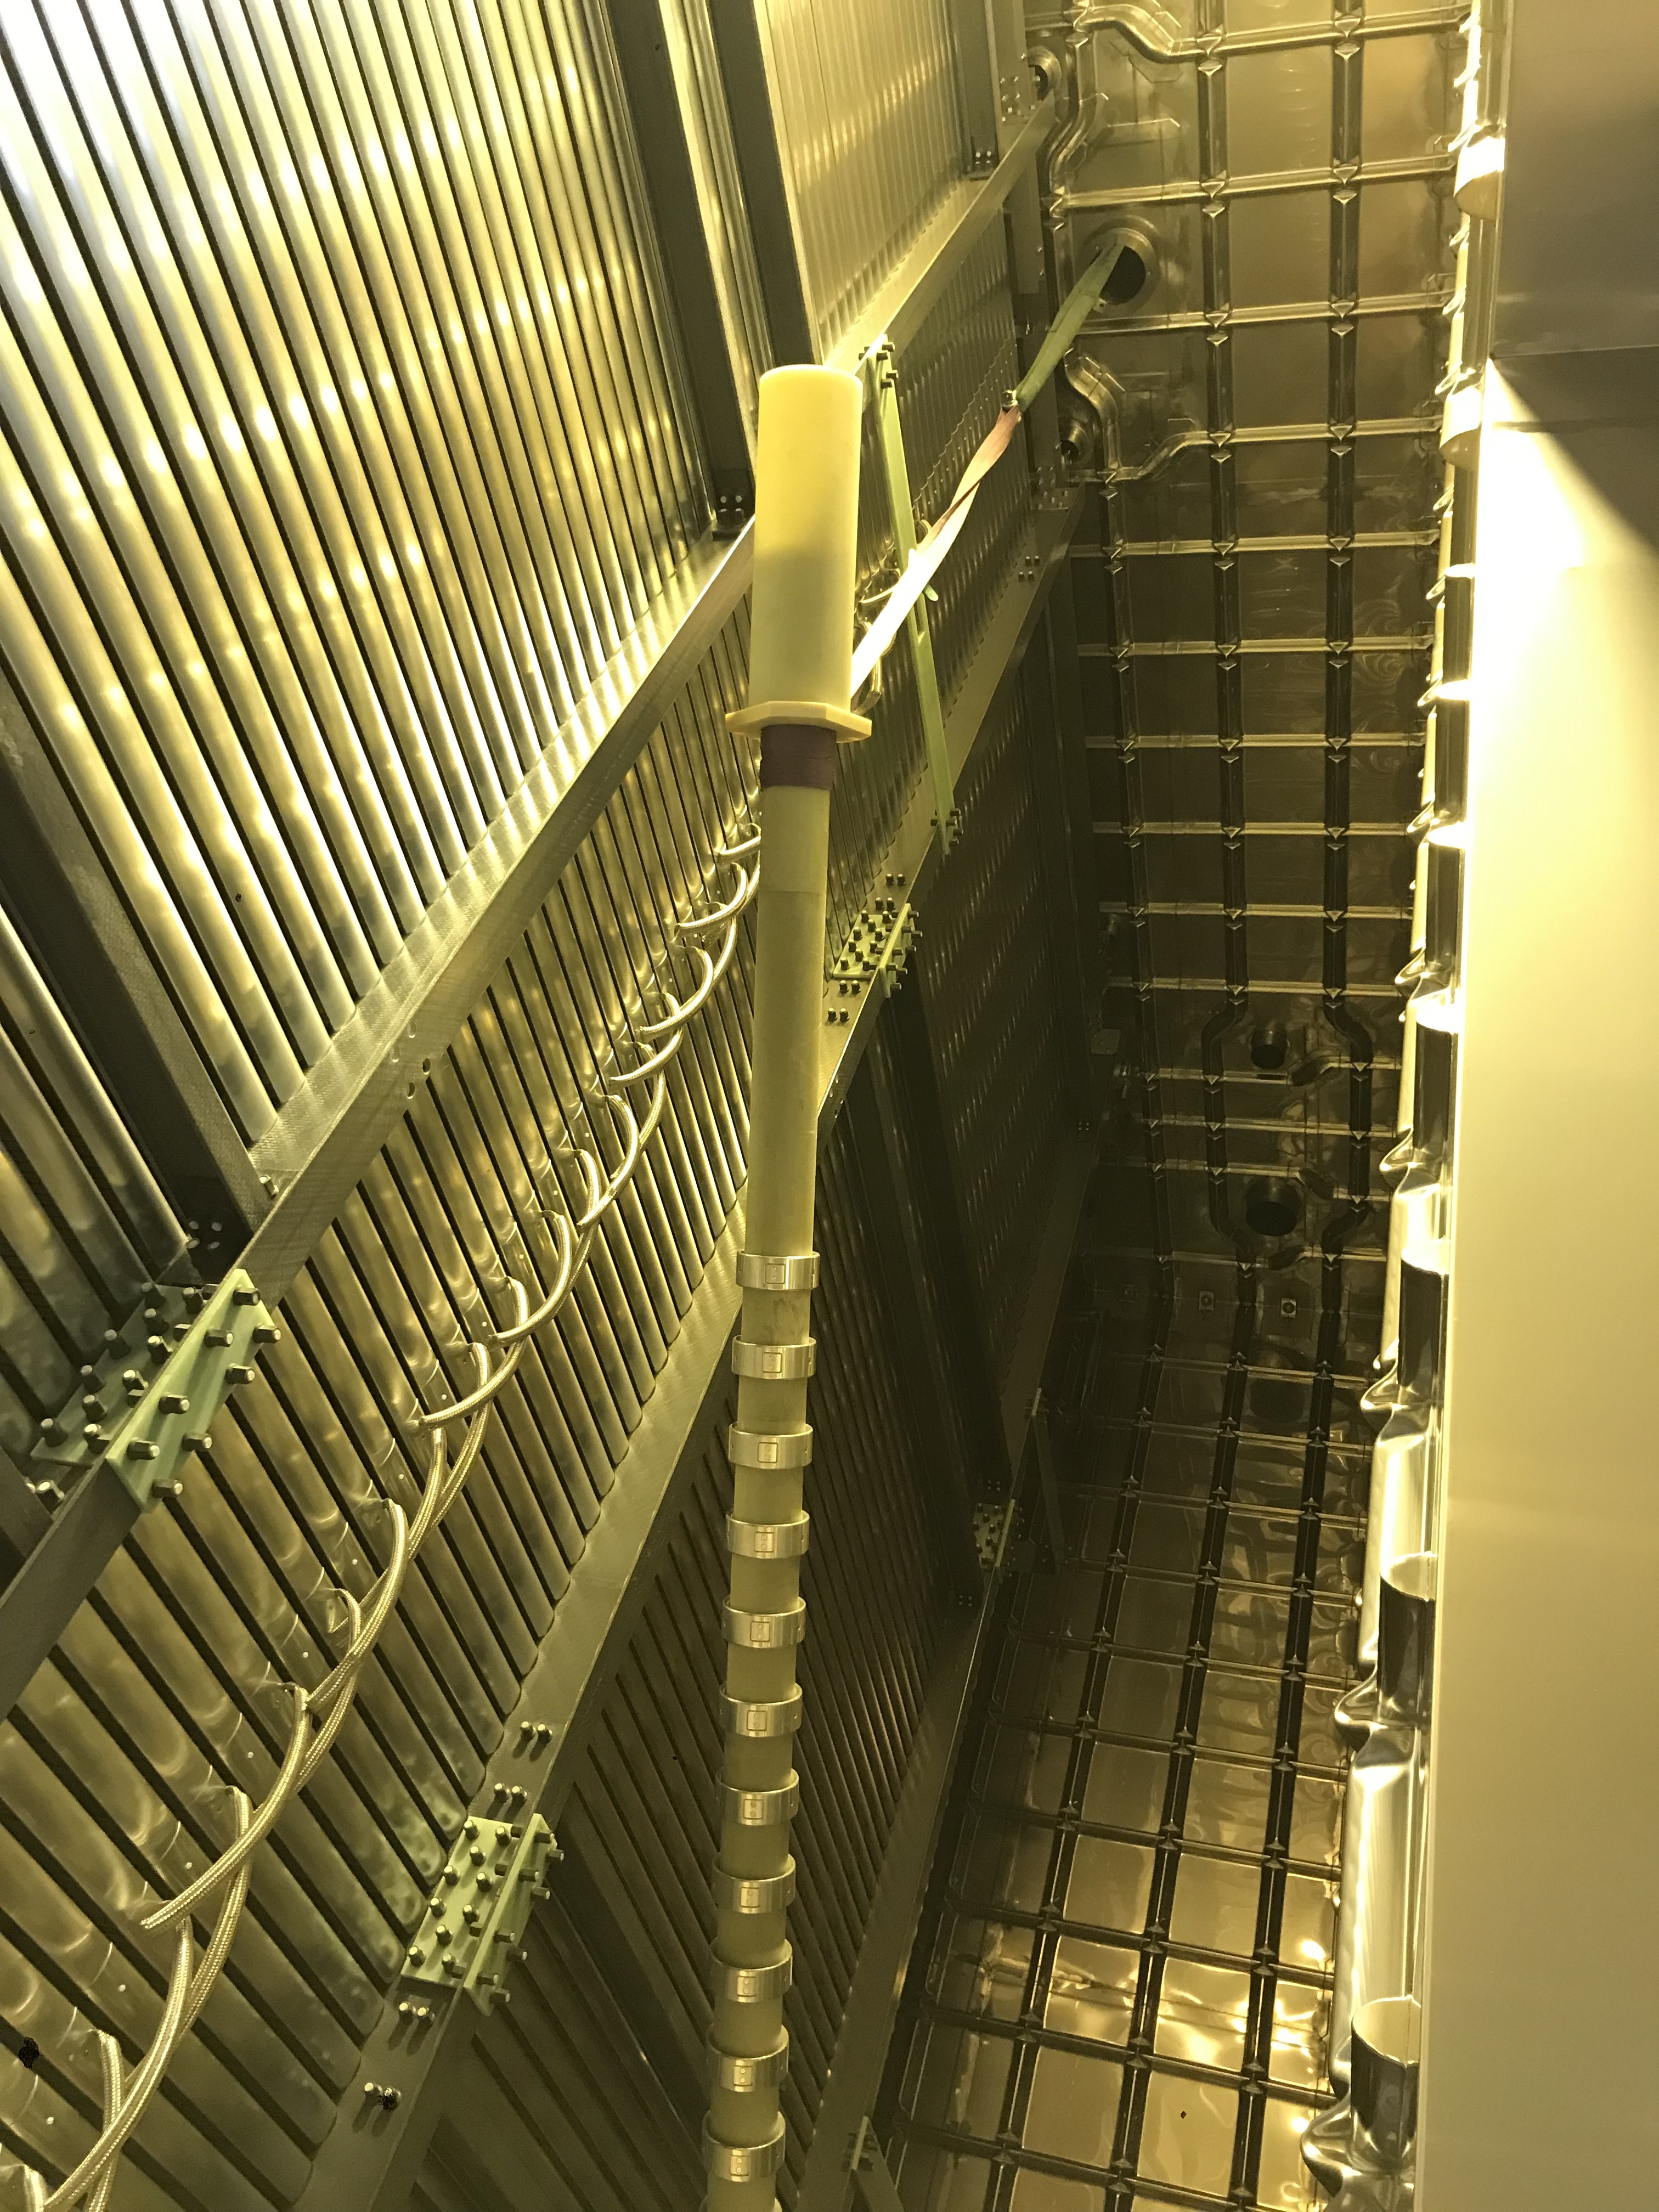
\includegraphics[width=0.9\textwidth]{extenderInstallation.jpg}
\end{dunefigure}



\subsection{Electronics installation}
The \dword{sgft} are installed and leak tested during the setup of the cryostat roof.
They must be available before the installation of the \dwords{crp} to connect the signal cables.
The \dword{fe} cards are mounted on the blades and inserted into the \dwords{sgft}.
The installation of the digital electronics and $\mu$TCA crates must be done once the infrastructure on the cryostat roof is completed.
This is mainly to prevent that ongoing work may damage the crates and the fibers connected to them.
Once the $\mu$TCA crates are installed and all the digital cards are inserted, the \dwords{amc} are cabled to the warm flanges of the \dword{sgft} for the charge readout, then connected to the \dword{pmt} signal cables for the light readout.
Finally, the 10~Gbit/s and 1~Gbit/s optical links to the \dword{daq} and \dword{wr} timing network are connected.

Given the presence of the cryogenic mezzanine and the unavailability of an overhead crane that can reach any position of the cryostat roof, the installation of the \dword{sgft} requires a compact gantry crane that can be moved on temporary rail or on wheels following the cryostat I-beams.
This part of installation will follow the welding of the corrugated membrane of the ceiling of the cryostat.
Sufficient amount of boxes containing the \dwords{sgft} must be stored underground.
The opening of the boxes is done on the cryostat roof.
After visual inspection, the \dwords{sgft} will be cleaned, hoisted with the gantry, inserted in the penetration and finally the CF flanges tightened.
Provided the availability of the material on the cryostat roof, two people can install eight \dwords{sgft} per shift. 
It will be crucial to test, possibly during the initial phase of the installation of the insulation that the penetrations are fulfill the requirements in terms of dimensions and linearity.
It is also important during the production of the \dword{sgft} to guarantee that all the pipes meet the requirements.
At \dword{pddp} the deformations of the penetration pipes due to welding and the dimensional non-conformity of few \dword{sgft} pipes resulted in delays of installation.
In parallel to the installation of the \dwords{sgft}, the \dword{fe} cards are unpacked on the cryostat roof, mounted on the blades on tables present for this purpose.
The instrumented blades are finally instrumented inserted in the \dword{sgft} before its sealing.
At this point, if the gas nitrogen pipes to purge the \dwords{sgft} are available they can be connected.
The sensors and the valves that potentially\footnote{It is not defined yet whether each \dword{sgft} needs independently temperature and pressures sensors and valves to control the gas nitroge flow.} needed to control the operation of the \dwords{sgft} can also be connected at this stage.
The installation of the $\mu$TCA crates with the digital electronics occurs in the final stage of the \dword{dpmod} installation to avoid damaging fragile equipment due to high level of co-activity expected on the cryostat roof for few months after the access to the top is granted.
The crates are placed and fixed in their designated positions on the cryostat roof.
They are connected to the power distribution network.
The \dword{amc} cards and \dword{wrmch} modules are inserted into their slots.
The connection of the \dword{cro} \dwords{amc} to the warm flange interface of the \dword{sgft} chimneys is done.
The optical fibres from the timing system are finally connected to the \dword{wrmch}.

The \dword{sgft} chimneys are commissioned first. This consists of evacuating their inner volume then filling the chimney with nitrogen gas at over-pressure between 5~mbar to 50~mbar.
The leak rate must be checked when the \dword{sgft} is under vacuum, and the nitrogen pressure must be monitored once the chimney is filled to verify that no damage occurs to the flange interfaces during installation.
Once the \dwords{sgft} are filled with gas nitrogen, the pressure must be constantly monitored and controlled.
It is crucial to monitor the \dword{sgft} pressure during the cryostat cool-down and filling.

The electronics system is commissioned after the $\mu$TCA crates,together with the \dwords{amc} and cabling the \dword{wr} network for the timing synchronization, are installed.
Functionality of the full \dword{daq} system is not strictly required at this stage.
The data from each crate is read with a portable computer connected to the crate using either the \dword{mch} 10~Gbit/s or 1~Gbit/s interface.
Non-functioning channels are identified by pulsing the CRP strips, and the data quality is examined to ensure the correct functioning of the digital electronics and the temporal alignment of the data segments.

\subsection{Light readout installation}

720~cryogenic Hamamatsu R5912-MOD20 \dwords{pmt}, below the transparent cathode structure, will be fixed on the membrane floor in the areas between the membrane corrugations.
The arrangement of the \dwords{pmt} accommodates the cryogenic piping on the membrane floor, and other elements installed in this area.
The attachment is done via a stainless steel support base point-glued to the membrane via four adhesive injection holes.
This fixation method will be long-term tested in cryogenic conditions prior the actual installation.
The installation of the \dword{pmt} will be done in sectors of 36~\dwords{pmt}, corresponding to the area below four \dwords{crp}, at a rate of 30~\dword{pmt}/week.
The \dwords{pmt} in each sectors will be installed, connected with cables and fibres, the connectivity will be tested, and finally the \dword{pmt} will be protected until the closure of the \dword{tco}. 

The \dwords{pmt} will be packed in individual boxes with their powering bases, support structures and short \dword{hv} cables soldered to the bases.
For shipping to \dword{ctsf} (probably located in the \dword{sdwf}), 36~\dwords{pmt} will then be placed in the transport boxes.
Following the \dword{ctsf} operations, the \dwords{pmt} will be placed in a custom structures in $4 \times 3$~arrays that can be moved into the clean room underground.
For transportation is done in boxes with three of these custom structures, for a total of 36~\dword{pmt} every box.
Excluding spares 20~boxes are needed to transport the 720~\dwords{pmt}.
The 80~spare \dwords{pmt} will be placed in three boxes, which can be stored in the \dword{ctsf}.
To maintain the cleanlyness inside the clean room underground, during tranportation the boxes will be wrapped with plastic that is then removed before entering into the clean room.
The entire $4 \times 3$ structure will go in the dark box for the final functionality tests.
The $4 \times 3$ array will be moved with the crane into the cryostat, placed on the cryostat floor, moved with trans-pallet at a convenient location for the installation, finally each \dwords{pmt} will be installed individually.

At the \dword{ctsf}, the \dwords{pmt} will be coated with \dword{tpb} at a rate of about 20~\dwords{pmt}/week.
The operations in the \dword{ctsf} should start enough in advance to secure sufficient availability of \dwords{pmt} during installation.
The \dword{ctsf} has sufficient storage capacity for the entire photon detector system of the \dword{dpmod}.

The weight of the support and the \dword{pmt} is approximately 7~kg.
Weight force exceeds the buoyancy force, still the assembly is light enough to be installed manually one at the time.
Given the large standing surface of the stainless steel plate, these supports ensure stability against possible lateral forces acting on the \dword{pmt}, for instance due to the liquid argon flow.

The support frame structure mainly comprises 304L stainless steel with some small Teflon parts.
The design takes into account the shrinking of the different materials during the cooling process to avoid breaking the \dword{pmt} glass.
The installation of an individual ground grids mechanically attached to the \dword{pmt} supports is also under consideration by the \dword{hv} and \dword{pd} system consortia.

Transport and storage of the cables and fibres are not an issue.
The cables and fibres arrive underground in boxes and they do not need to be cleaned before installation.
The cryostat cable/fiber installation will precede the installation of the \dword{fc}.
The cables/fibers will be routed from the relevant flanges to the bottom of the cryostat, with the help of dedicated cable trays and support from the cryogenic cooling pipes along the long walls.
Work at height will be carried out using the man lifts.
The free ends of the cables/fibers will be temporarily secured to the cryostat floor so they can be easily accessed during installation.
Once the temporary floor is removed, the ground grids set in high position and the \dwords{pmt} placed in their final position, the short \dword{hv} cables will be connected to the one coming from the feedthrough and the calibration fibers will be routed and connected to the support structure.
The fixation of the cables and fibres will be done at the level of the \dword{pmt} supports and on the ground grids.

\subsection{\dshort{tco} closure}
The activities related to the \dword{tco} closure involve heavy and dirty work, like grinding and welding, also inside the cryostat.
At that time, all the large detector components must be inside the cryostat including the material for the completion of the thermal insulation and the primary membrane.
The cryostat will be defined as a confined space, a work area with difficult egress.
The access will be limited and only from the available man-holes.
In order to access, scaffold is a solution being studied.
The height and the width of the volume between the \dword{fc} and the cryostat wall will require a special scaffold.
Alternatively, an electric pulley can be used to bring in and out material and personnel, by means of harness, that should anyway be used in a confined space.

Most of the detector will actually be installed, including the \dword{fc} end-wall in the proximity of the \dword{tco}.
This is the approach used in the \dword{pddp} case.
It is therefore mandatory to protect the cryostat, that should be considered as an ISO~8 class clean room, and the detector components.
A dirty room made out of aluminium profiles, plywood panels (treated with fire retardant agents) and fire retardant plastic sheets will be constructed in the area between the cryostat wall and the \dword{fc} end-wall.
Such a room was built in less than two week by four technicians inside the \dword{pddp}.
Since the access and the dirty room volume is similar to \dword{pddp}, the time and man power will be the same.
The engineering of the insulation and the primary membrane as not yet finalized, so the dimensions of the insulation panels and corrugated membrane needed for the \dword{tco} closure is not yet defined.
The dirty area anyway will be done large enough to store all the insulation panels needed.
They will be arranged in the correct installation order, because due to tight space it will be difficult to swap two panels.
The need of a scaffold in front of the \dword{tco} in order to be able to install the topmost panels is unavoidable.
The actual installation of the insulation and the primary membrane will most likely be carried out by the same company that installed the rest of the cryostat.
In the \dword{pddp} case this operation took less than four weeks and five people.
Again, the time estimation to complete this work in \dword{dpmod} is similar to the \dword{pddp} case.
The cleaning and the removal of the dirty room finally is done in the last two weeks dedicated to the \dword{tco} closure activities.

The last month of activities inside the cryostat is dedicated to complete the installation of the remaining cryogenic instrumentation, clean the cryostat and the accessible detector components, remove all the equipment needed for access and close finally the man-holes.
